% ****** Start of file apssamp.tex ******
%
%   This file is part of the APS files in the REVTeX 4.2 distribution.
%   Version 4.2a of REVTeX, December 2014
%
%   Copyright (c) 2014 The American Physical Society.
%
%   See the REVTeX 4 README file for restrictions and more information.
%
% TeX'ing this file requires that you have AMS-LaTeX 2.0 installed
% as well as the rest of the prerequisites for REVTeX 4.2
%
% See the REVTeX 4 README file
% It also requires running BibTeX. The commands are as follows:
%
%  1)  latex apssamp.tex
%  2)  bibtex apssamp
%  3)  latex apssamp.tex
%  4)  latex apssamp.tex
%
\documentclass[%
 reprint,
%superscriptaddress,
%groupedaddress,
%unsortedaddress,
%runinaddress,
%frontmatterverbose, 
%preprint,
%preprintnumbers,
%nofootinbib,
%nobibnotes,
%bibnotes,
 amsmath,amssymb,
 aps,
%pra,
prb,
%rmp,
%prstab,
%prstper,
%floatfix,
]{revtex4-2}

\usepackage{graphicx}% Include figure files
\usepackage{dcolumn}% Align table columns on decimal point
\usepackage{bm}% bold math
\usepackage{hyperref}% add hypertext capabilities
\hypersetup{colorlinks=true,urlcolor={blue},citecolor={blue}, linkcolor={blue}}
\usepackage{amsmath} % or simply amstext
%\newcommand{\angstrom}{\textup{\AA}}
\usepackage{siunitx}
\usepackage{color}
%\usepackage{url}            % simple URL typesetting
%\usepackage[mathlines]{lineno}% Enable numbering of text and display math
%\linenumbers\relax % Commence numbering lines
%\usepackage{nameref}

%\usepackage[showframe,%Uncomment any one of the following lines to test 
%%scale=0.7, marginratio={1:1, 2:3}, ignoreall,% default settings
%%text={7in,10in},centering,
%%margin=1.5in,
%%total={6.5in,8.75in}, top=1.2in, left=0.9in, includefoot,
%%height=10in,a5paper,hmargin={3cm,0.8in},
%]{geometry}

%RZK: do not edit red text
\newcommand{\lock}{\color{red}}

\begin{document}

\preprint{APS/123-QED}

\title{Adatoms in the surface Ullmann coupling}% Force line breaks with \\
%\thanks{A footnote to the article title}%

\author{Zhenzhe Zhang}
 %\altaffiliation[Also at ]{Physics Department, XYZ University.}%Lines break automatically or can be forced with \\
\author{Dmitrii F. Perepichka}%
 %\email{dmitrii.perepichka@mcgill.ca}
\author{Rustam Z. Khaliullin}
 %\email{rustam.khaliullin@mcgill.ca}
\affiliation{%
 Department of Chemistry, McGill University,\\ 801 Sherbrooke St West, Montreal, QC H3A 0B8, Canada
 %This line break forced with \textbackslash\textbackslash
}%

%\date{\today}% It is always \today, today,
             %  but any date may be explicitly specified

\begin{abstract}
This manuscript reviews the results of experimental and computational studies of the surface Ullmann coupling that shed light on the role of surface adatoms in its mechanism. A particular focus is on the early stages of the polymerization and coupling of two monomers.
\end{abstract}

\maketitle

%\tableofcontents

%RZK. What a variety of RZK labels mean. 
%R1111 or RZKmmdd - mm denotes month, dd - denotes day
%RZKX - these are low priority comments, which will be promoted to regular labels later 
%RZZK - ignore! These labels keep track of my own revision process

%%% GENERAL REMARKS %%%

%RZK: Do not mention the year of publication if you do not describe the history of research. Do not mention authors unless this is important.

%RZK: I have stated this before and I have to emphasize this one more time that you should use PRESENT PERFECT tense, not PAST SIMPLE when you report previous findings. Do not use PAST tense to report hings that are universally TRUE, use PRESENT SIMPLE. For example, "The energy barriers follow", not ""The energy barriers followed"

%RZK: Detailed description of the figure. Take a look at the original publication. Reprinted from~\cite{RZK} with permission of American Chemical Society or PUBLISHER. See the LaTeX comment below. If you take a figure from a publication it is very important to cite the work and obtain publisher's permission. We need to make sure that all our borrowed figures satisfy copyright permissions. For example, see: https://www.stm-assoc.org/2016_01_05_Guidelines_for_Quotation_From_Journal_Articles.pdf

%RZK. Use Figure instead of Fig. in your text.

%RZK: Do not capitalize names of elements.

%RZK1221: Do not use math mode to emphasize text. Use \emph{text}.

\section{Introduction}

%RZK0108: The lock on the first sections is lifted so Dima can see it in black. Your modifications should be inserted in blue.

\subsection{Ullmann coupling in solution}

In 1901, Fritz Ullmann discovered~\cite{ullmann_01} a coupling reaction that creates a C--C bond between aryl halide molecules in the presence of a stoichiometric amount of Cu powder. 
%Currently, the scope of Ullmann coupling reaction is being widened with an increasing number of substrates, leaving groups, and active metal species being investigated for constructing various C--X bonds. 
Because of its ability to form C--C bonds, Ullmann coupling has become one of the key reactions in organic synthesis with its scope extended to new reactants and catalysts. 
Today, the \emph{classical} Ullmann or simply Ullmann reaction refers to a family of nucleophilic substitution reactions between aromatic nucleophiles that proceed in the presence of copper and lead to the formation of C--C and C--heteroatom bonds such as C--N~\cite{ullmann_02, ullmann_03}, C--O~\cite{ullmann_04}, C--S~\cite{ullmann_05} and C--P~\cite{ullmann_21,ullmann_22} bonds (Fig.~\ref{fig:UllmannCoupling}). 
%RZZK: In Ullmann coupling, metals can serve as reactants or as catalysts.

\begin{figure}[htb]
\centering
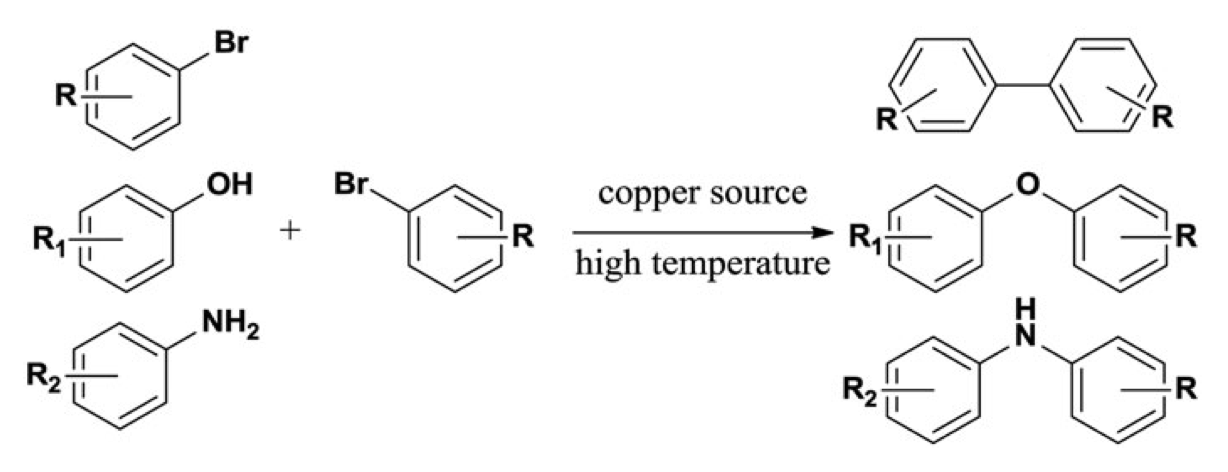
\includegraphics[width=0.90\columnwidth]{Fig/classical.png}
\caption{Examples of the Ullmann coupling reactions.}
\label{fig:UllmannCoupling}
\end{figure}

Depending on the type of bonds created, reactants in the Ullmann coupling can be aromatic amines~\cite{ullmann_17,ullmann_18}, amides~\cite{ullmann_19,ullmann_20}, phosphines~\cite{ullmann_21,ullmann_22}, carboxylic acids~\cite{ullmann_23}, diaryl ethers~\cite{ullmann_24}, phenols~\cite{ullmann_25} and other oxygen-containing species~\cite{ullmann_26,ullmann_27,ullmann_28}. 
While halides, especially iodides and bromides served as typical leaving groups, the usage of the tosylate leaving group has also been reported~\cite{ullmann_15}. 
Cu-containing compounds are most widely used as activating agents. In addition to traditional Cu(0), different Cu(I) and Cu(II) salts and oxides -- including CuI~\cite{ullmann_07,ullmann_08,ullmann_09}, CuBr~\cite{ullmann_10,ullmann_11}, CuCl~\cite{ullmann_13}, Cu$_2$O~\cite{ullmann_12}, Cu(acca)$_2$~\cite{ullmann_14}, Cu(OTf)$_2$~\cite{ullmann_15}, CuO~\cite{ullmann_16} -- have been used {\color{blue}as well}. 
Apart from Cu agents, Pd nanocomplexes~\cite{ullmann_35, ullmann_36}  have been proven effective in the Ullmann coupling reaction. 

Ullmann coupling has been acquiring greater significance in the last decade because Cu is a cheaper alternative to Pd, Pt and Rh, because halogen side-product can be avoided and because air or oxygen can act as oxidants~\cite{ullmann_38,ullmann_39,ullmann_40,ullmann_41}. Despite widespread applications, Ullmann reaction suffers from several limitations including the necessity of high temperature and polar solvents with high boiling point, low solubility of many Cu compounds, erratic yields, and poor functional group tolerance leading to a limited substrate scope~\cite{ullmann_31}. %Apart from this, the usage of Cu does not meet the prerequisite of sustainable development.

The mechanism of classical Ullmann coupling is relatively well understood (Fig.~\ref{fig:classical}).
It is widely accepted that an aryl halides molecule reacts with Cu species to form an organometallic intermediate. This intermediate then reacts with a second aryl molecule through oxidative addition producing a diaryl organomitallic intermediate, which subsequently undergoes reductive elimination to form a covalent bond between the two aryls. 
%The Ullmann coupling reactions discussed above occur mostly in organic solvents. 

\begin{figure}[htb]
\centering
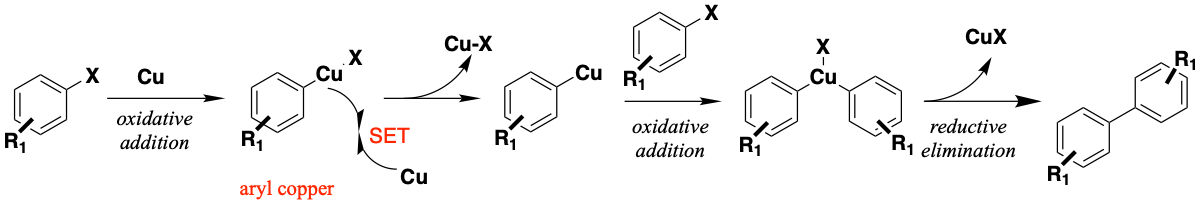
\includegraphics[width=1.0\columnwidth]{Fig/ullmann_mechanism.png}
\caption{Mechanism of the Ullmann coupling reaction. SET stands for single-electron transfer.
}
\label{fig:classical}
\end{figure}

Recent advances in the classical Ullmann coupling reaction have been reviewed by several authors~\cite{ullmann_29,ullmann_30,ullmann_31,ullmann_32}.

\subsection{Surface Ullmann coupling}

A recent surge of interest in electronic devices based on low-dimensional organic nanostructures with $\pi$-conjugated backbones has led to a renewed attention to the Ullmann coupling reaction. 
In the case of low-dimensional materials, the well-established ability of Ullmann coupling to create bonds between aromatic carbon atoms and couple their $\pi$ systems have been transferred from solution to metal surfaces, which serve as both a low-dimensional confining template and catalyst.

The on-surface Ullmann reaction is currently viewed as a promising bottom-up strategy to assemble, in mild conditions, one- and two-dimensional organic polymers with high degree control of their electronic properties~\cite{ullmann_33}. 
In the context of surface reactions, the term Ullmann coupling has been extended to refer to the reaction on metals other than copper, such as silver and gold. 

One of the first fundamental studies of the surface-confined coupling of iodobenzene to biphenyl under ultrahigh vacuum (UHV) condition was reported by Xi and Bent~\cite{sur_sci01} in 1992.
%
The intermediate species of the same reaction were inspected using STM imaging by Weiss \textit{et al.}~\cite{langm01} in 1998. 
In 2004, it was demonstrated that linear \emph{protopolymers}---aligned monomer units of a polymer that have not yet reacted to form the final polymer---could be obtained by depositing \textit{para}-diiodobenzene on Cu(111) at 77 K~\cite{jacs01}. 
This insight showed that the Ullmann coupling can be used not only to synthesize organic molecules but periodic polymers as well.
Remarkably, the first synthesis of covalently-bonded nanostructures from molecular building blocks on metal surfaces under vacuum has employed the Ullmann reaction: the coupling between brominated tetraphenyl-porphyrins on the Au(111) surface was performed by Grill \textit{et al.}~\cite{Naturenano2007} in 2007.

Since then, surface Ullmann coupling has become one of the most representative on-surface synthesis schemes. It has been utilized to create covalently-linked extended aromatic systems on a variety of metal surfaces starting from halogenated aryl precursors~\cite{ullmann_33,ullmann_34, ullmann_42, ullmann_43, ullmann_45, ullmann_46, ullmann_47, ullmann_48}. 

\subsection{Mechanism of surface Ullmann coupling}

Although multiple covalently-bonded nanostructures have been obtained on metal surfaces via Ullmann coupling, our knowledge of the mechanism of the surface processes still remains fragmentary. 
A thorough understanding of the mechanism of surface Ullmann coupling reaction will enable rational, faster, more precise design of the halogenated precursors, well-matched to a chosen metal surface.
The overall coupling process can be divided into elementary steps depicted in Fig.~\ref{fig_mecha} and described in details below. It should be noted that the surface Ullmann coupling proceeds through the formation of the organometallic intermediates similar to those encountered in the reaction in solution (Fig.~\ref{fig:classical}).

The focus of the following review of the Ullmann coupling mechanism is entirely on the formation of a carbon-carbon bond from halogen-containing precursors on Cu, Ag and Au surfaces. A particular attention is paid to the monohalogenated benzenes. 

\begin{figure*}[tb]
\centering
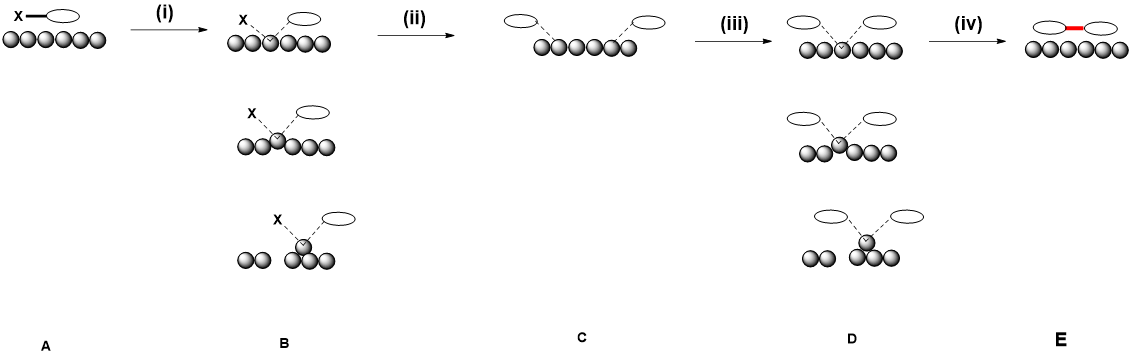
\includegraphics[width=0.9\textwidth]{Fig/mechanism.png}
\caption{Schematic represnetation of elementary steps of a surface Ullmann coupling process. RZK0108: This figure needs further discussion.}
\label{fig_mecha}
\end{figure*}

%%\begin{enumerate}[align=left, itemindent=2em, label=(\roman*)]
    %%\item Dehalogenation of Precursors [The fundamental step is the %%disassociate of halogens, the cleavage of C-X bonds (X = halogens) is %%usually activated by thermal, electron-induced and photon-simulated. %%The energy will vary from 0.05 ~ 0.80 eV with different X on different %%coinage surfaces.]
    %%\item Diffusion of single Dehalogenlated 'Radicals' [The removal of %%halogens from precursors results in unsaturated carbons (radicals), %%which interact with metal atoms to form C-Metal radical (C = %%dehalogenated precursor and Metal = Au, Ag or Cu). C-Metal radical %%will diffuse on metal surface and the metal atom interacting with the %%radical will shift.]
    %%\item The Formation of Organometallic Intermediates C-Metal-C from Two %%Single Radicals [Diffusion brings two single radical close to each %%other, and then these two species would form a dimerized %%organometallic intermediate before the appearance of coupling product]
    %%\item The Formation of Carbon-Carbon Bond []
    %%\item Diffusion of Coupling Product []
%%\end{enumerate}  


\subsubsection{Dehalogenation}

{\lock

The first fundamental step of surface Ullmann coupling is the dissociative dehalogenation of organic precursors adsorbed on the surface. In this step, the carbon-halogen bonds of the precursor are broken whereas the carbon-metal and halogen-metal bonds are formed. The thermodynamics and kinetics of the process are primarily determined by the relative strength of the broken and formed bonds. 

}%lock

RZK0108: This subsection needs more work following the guidelines discussed in December. Trends in experimental data should be presented first, desirably for Ph-X. Your review will be particularly strong if the trends are discussed across all three metals and three halogens for Ph-X. After experiments, discuss if the trends can be reproduced from simple bond-strength models. Then, present a short summary of DFT calculations to say if the experimental trends can be reproduced using electronic structure methods. I only rearranged your text a bit, you must work on it extensively.

The following data illuminates the strong influence of surfaces and halogens on the first step of the Ullmann coupling of two Ph-X. For instance, the dissociaton of iodobenzene occurs at \SI{175}{\kelvin} on Cu(111)~\cite{sur_sci01}, \SI{200}{\kelvin} on Ag(111)~\cite{sur_sci02} and \SIrange{200}{250}{\kelvin} on Au (111)~\cite{sur_sci03}. 
The same trend has been observed for bromobenzene with a higher temperature on all surfaces. RZK0122: Find temperatures for bromo and chloro-benzene. 

RZK0122: The following paragraph is taken from your mechanism summary. It should be discussed here instead. 

The dehalogination of other organic precursors follow the same trends observed for Ph-X. it has been observed that the reactivity trend decrease in the order Ar--I $>$ Ar--Br $>$ Ar--Cl both in experiment and theoretically~\cite{ullmann_52}. This also means that the dissociation of Ar--I bond on metal surface requires the lowest temperature. In addition, the energy barrier of dehalogenation is the highest on Au(111) surface, the lowest on Cu(111) surface both in experiment and in theoretical calculations~\cite{jacs2013}. It has also reported that the miller index of metal surface will also influence the reaction energy of dehalogenation~\cite{ullmann_57}. 

To explain the observed differences in reactivity, the following trends in the bond strength have been derived from model molecular systems.
%
\begin{eqnarray}
\begin{split}
\text{C--Cl} > \text{C--Br} > \text{C--I} \\ 
\text{Cu--C} > \text{Au--C} > \text{Ag--C} \\
\text{Cu--Cl} > \text{Cu--Br} > \text{Cu--I}\\
\text{Ag--Cl} \approx \text{Ag--Br} > \text{Ag--I} \\
\text{Au--Cl} > \text{Au--I} > \text{Au--Br}
\end{split}
\end{eqnarray}
%
The bond dissociation energy of diatomic and CX$_4$ molecules have been used in the cases of the metal-halogen bonds~\cite{ullmann_62} and carbon-halogen bonds~\cite{ullmann_63}, respectively. The relative strength of metal-carbon bond strength has been estimated using the metal-carbon bond distances in M-(CH$_3$)$_2$ molecules~\cite{ullmann_61}.

By combining the strength of all metal-halogen bonds shown above the following series emerges
%
\begin{gather*}
\text{Cu--Cl} > \text{Cu--Br} > \text{Au--Cl} \approx \text{Au--I} \approx \text{Ag--Br} \approx \\
 \approx \text{Ag--Cl} > \text{Ag--I} > \text{Au--Br} > \text{Cu--I}
\end{gather*}
%

RZK0108: Why you are ordering the strength of metal-halogen bonds? Is it uselful for predicting of the kinetics of the first step (i.e. reaction temperature)? I do not expect this trend to be suitable for the thermodynamics that is certainly affected not only by M-X strength but also by C-X and C-M strengths. We need to predict the energy of this step: C-X bond is broken, C-M bond is formed, X-M bond is formed. Has it been done in any review articles?

DFT calculations have estimated the activation barrier for the exothermic dehalogenation of bromobenzene and iodobenzene on (111) metal surfaces to be \SIrange{0.4}{1.0}{\electronvolt}~\cite{jacs2013}. As shown in Fig.~\ref{fig:dehalo}, the activation barrier and reaction energy decrease in the order Au $>$ Ag $>$ Cu and are \SIrange{0.1}{0.5}{\electronvolt} lower for iodobenzene than bromobenzene. The latter is due to the dissociation energy of a C--I bond being $\sim$\SI{0.65}{\electronvolt} lower than that of a C--Br bond~\cite{Arpc1982}. RZK0123: Any data on chlorobenzene?

\begin{figure}[tbh]
\centering
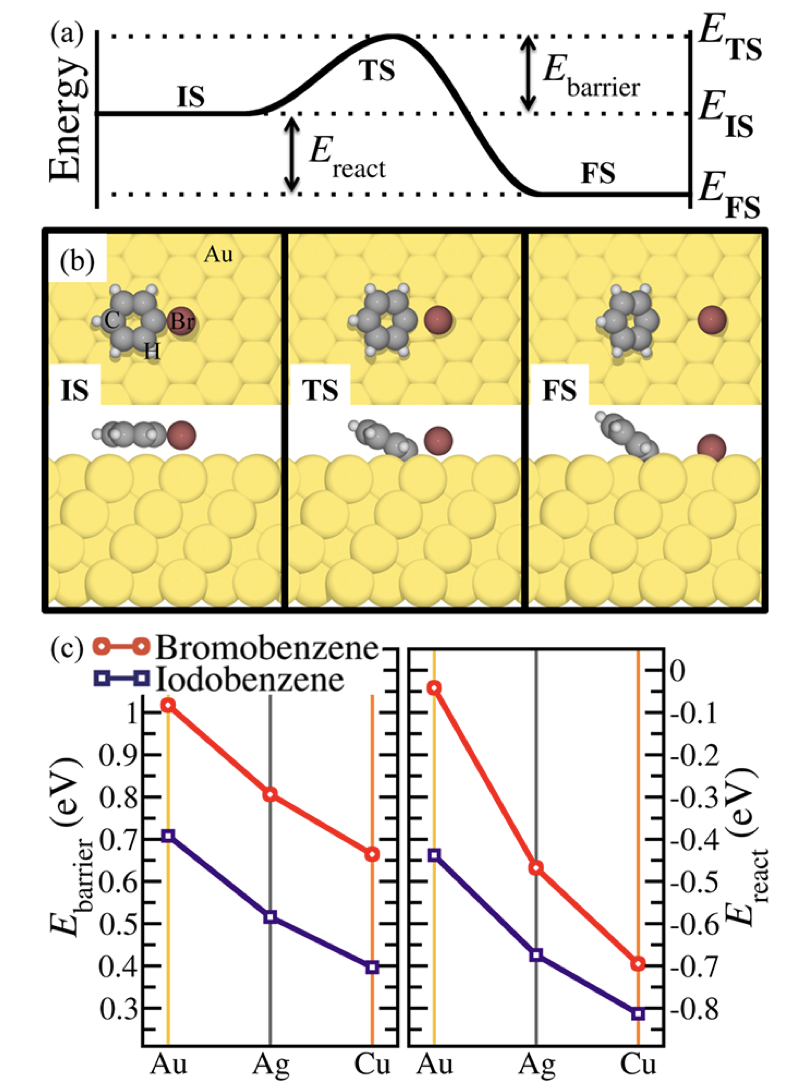
\includegraphics[width=0.75\columnwidth]{Fig/dehalogentaion.png}
\caption{(a) Definitions of the energy barrier ($E_{barrier}$) and reaction energy ($E_{react}$) for dehalogenation reactions. (b) The dissociation of bromobenzene on Au(111), depicting top and side views of the initial state (IS), transition state (TS), and final state (FS) of the reaction. (c) $E_{barrier}$ (left) and $E_{react}$ (right) for the dissociation of bromobenzene and iodobenzene on the (111) facets of Au, Ag, and Cu.} 
\label{fig:dehalo}
\end{figure}

\subsubsection{Diffusion}

{\lock

The dehalogenation step produces organometallic intermediates with carbon atoms covalently bonded directly to surface metal atoms. 
The diffusion of these species, which has been observed experimentally and studied computationally, plays a decisive role in the further coupling process. 
A high mobility of molecules increases the chances of two molecules moving closer to each and forming a bond. Therefore, low energy barriers for diffusion process are a prerequisite for the self-assembly of well-ordered networks

Among dehalogenated precursors, the diffusion of a phenyl group has been studied most thoroughly. 
Computational studies have considered sliding or flipping mechanisms of diffusion~\cite{pccp2010, jacs2013}. 
In the sliding diffusion, a phenyl group keeps its orientation to the surface in the initial, transition and final states. The energy barrier of the sliding diffusion on (111)metal surfaces decreases from \SI{0.44}{\electronvolt} on Cu to \SI{0.29}{\electronvolt} on Ag and to \SI{0.22}{\electronvolt} on Au. 
In the flipping diffusion, a phenyl group increases its tilting angle, achieves the upright configuration and then overturns to bind to an adjacent metal atom. 
For this diffusion mechanism, the change in the magnitude of the diffusion barriers follows a different trend and decreases from \SI{0.19}{\electronvolt} on Au to \SI{0.07}{\electronvolt} on Cu and to \SI{0.06}{\electronvolt} on Ag. 
The low calculated barriers agree with STM studies that have revealed that dehalogenated phenyl groups diffuse on the Cu (111) surface at temperatures as low as \SI{77}{\kelvin}~\cite{langm01}. 

It should be noted that the flipping diffusion may not contribute significantly for larger precursor molecules, especially those anchored to the surface by several covalent bonds. The stronger surface-molecule interaction will favor diffusion mechanism with the molecular plane remaining parallel to the surface~\cite{ullmann_65}.

%RZZK: This is from jacs2013
%Furthermore, the presence of Cu adatoms may impact the self-assembly more than the poor diffusion on the atomically flat Cu(111) surface. These adatoms are known to have a great influence on selfassembly on Cu(111), where in many cases coordination bonds are formed instead of covalent networks.21 The Cu adatoms can also contribute to the covalent bonding of the nanostructure.22,23

Halogen atoms chemisorbed on the surface also undergo the diffusion process. The binding energy of halogens and their diffusion barriers have been investigated using DFT calculations~\cite{jacs2013}, which show that halogens hop between fcc and hcp hollow sites with the transition state being the bridge site. The diffusion barriers for a variety of metal-halogen combinations have been found to be in the \SIrange{0.05}{0.1}{\eV} range, implying that the halogens are highly mobile on the three metal surfaces at experimental temperatures. The barrier tends to be largest on Au(111) and smallest on Cu(111). At high surface coverage, halogens atoms bonded to the surface might hinder the diffusion of organic precursors preventing them from approaching each other and hence slowing down the coupling process. 

%RZK0122: Should we add the following citation to the previous paragaph?
%There are few experiment works related to the diffusion of halogen atoms on metal surface, but it is much better investigated theoretically using DFT calculations~\cite{ullmann_66}.

%RZK0122: The following data can be added but only as a table, not text.
%Atomic bromine has been reported to have a diffusion energy barrier of \SI{0.09}{\electronvolt}, \SI{0.07}{\electronvolt} and \SI{0.06}{\electronvolt} on Au(111), Ag(111) and Cu(111) respectively. Atomic iodine have a barrier of \SI{0.11}{\electronvolt}, \SI{0.06}{\electronvolt} and \SI{0.06}{\electronvolt} on Au(111), Ag(111) and Cu(111) respectively. And atomic chlorine have a barrier of \SI{0.02}{\electronvolt} and \SI{0.08}{\electronvolt} on Au(111) and Cu(111) respectively. 

}

\subsubsection{Formation of carbon-metal-carbon intermediates} \label{sec:dimerized}
%RZZK: Dimerization??? (%ZZ two organometallic intermediates bond together)

{\lock

Dimerized organometallic intermediates form when two organic fragments diffuse close to each other and become bound to the same metal atom, without yet creating a direct covalent bond with each other. Since the distance between two carbon atoms in such carbon-metal-carbon bridges is significantly larger than in a covalent bond, their existence has been confirmed in multiple  STM and AFM experiments~\cite{jacs2011}, corroborated with computational studies.

STM images of phenyl groups on Cu(111) show that structures consisting of two groups bound to the same metal atom form at \SI{160}{\kelvin} (Fig.~\ref{fig:organ}). The measured geometry of these intermediate structures agree with those obtain from DFT modeling~\cite{ullmann_67}. The activation energy of forming such bridge structures from two single organometallic intermediates has been calculated to be \SI{0.38}{\electronvolt}~\cite{pccp2010}. 
%RZK0122: I cannot find the number you mentioned above in this article. This number means that the formation of dimerized species needs much higher activation energy than simple diffusion. Check this number.

%RZK0122: There is no reference in the following sentence. 
The existence of organometallic bridges has also been demonstrated for dibromoterphenyl on Cu(111) and Ag(111) surfaces at \SI{300}{\kelvin} by a combined STM and DFT study. 
%RZK0122: pDOS can confirm this existence only if combined with experiments. What kind of experiments? Reply in comments, do not re-write the text.
Projected density of states also indicates the existence of the organometallic bridge structures~\cite{jacs2011, PCCP2012}. 

%RZK0122: Read the paragraph, calrify in the comments, do not re-write text.
The observation of the bridge structures on both metals at \SI{300}{\kelvin} implies that the barrier for [RZK0122: the further C--C bond formation step][OR][the bridge formation] on Ag and Cu surfaces are similar. 
Compared to the dehalogenation, this step [RZK0122: which step? see above] requires between 150 and \SI{200}{\kelvin} higher temperature [RZK0122: higher than what?]. It is remarkable that while organometallic bridges are common on Cu and Ag surfaces they are only occasionally reported on the Au surface [RZK: reference]. This phenomenon is explained by a relatively low energy barrier for the C--C bond formation between precursors on the Au surface that results in a very short life-time of the bridges~\cite{ullmann_33}.

}


\begin{figure}[ht]
\centering
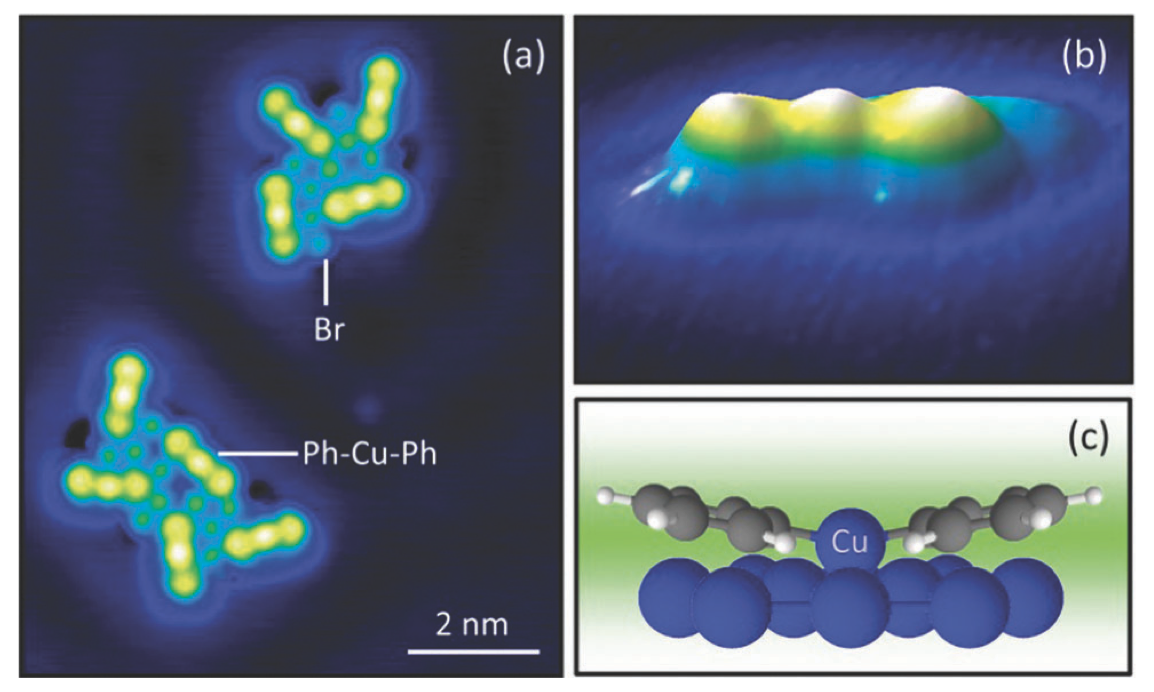
\includegraphics[width=0.85\columnwidth]{Fig/phenylorgano.png}
\caption{STM images and model showing the assembly and high-resolution details of the organometallic intermediate. Images are collected at \SI{5}{\kelvin}. Structures are formed at \SI{160}{\kelvin} (a) Clusters of the organometallic intermediates and Br atoms. (b) 3D rendering of a single phenyl–Cu–phenyl intermediate. (c) Model showing the bonding of two phenyl groups to the Cu atom.}
%RZK0122: looks like an adatom
\label{fig:organ}
\end{figure}


\subsubsection{Formation of the C--C bond}

{\lock

%RZK0122: Annealing can have different meaning. Use simpler word(s).
After further annealing[RZK0122: increase/decrease/changes in temperature], a covalent C--C bond is formed spontaneously and irreversibly between the two organic precursors anchored to the same metal atom. The structural changes in this elementary step as well as its energetics have been extensively studied using experiments and simulations.

} %lock

Biphenyl products are reported to form from two phenyl groups at \SI{350}{\kelvin} on Cu(111) surface in experiment~\cite{ullmann_68, ullmann_69}. 
RZK0122: The same experimental data for Ag and Au is necessary. This is the data mentioned in pccp2010 (references must be renumbered). The biphenyl formation temperatures are higher on Cu(111) (over 300 K) [5,6], and lower on Au(111) (165--180 K) [9] and on Ag(111) (110 K) [4].

In agreement with experiments, DFT calculations indicate that the formation the C--C bond for two phenyl groups is highly exothermic for all surfaces~\cite{jacs2013}. They also demonstrate (Fig.~\ref{fig:coupling}) that the energy change of this step decreases from RZK on Ag to RZK on Au and RZK on Cu whereas the energy barrier decreases from RZK on Ag to RZK on Cu and RZK on Au. 

\begin{figure}[ht]
\centering
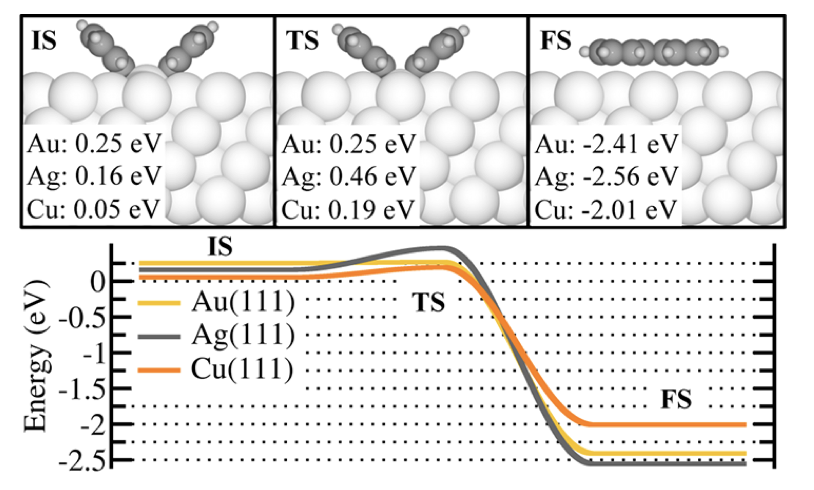
\includegraphics[width=0.75\columnwidth]{Fig/couplingenergy.png}
\caption{Energy diagram for the coupling reaction of two phenyls into biphenyl on the of Au(111), Ag(111), and Cu(111). In the top panel, the reaction is depicted for Ag(111), with the energy indicated for each of the states along the path for the respective surface. The energies are given with respect to the most stable adsorption configuration of an isolated phenyl on the respective surface.}
\label{fig:coupling}
\end{figure}

If organic monomers contain more than one functional group, the Ulmann coupling proceeds further with the formation of trimers~\cite{jacs2016}, oligomers~\cite{ullmann_53, ullmann_56} or polymers~\cite{ullmann_43, ullmann_54, ullmann_55}. DFT modeling of the dimerization and trimerization of 1,4-dibromobenzene on Cu(100) surface shows that the activation energy for the C--C bond formation is \SI{0.7}{\electronvolt} and \SI{0.2}{\electronvolt}, respectively~\cite{jacs2016}. The first energy value is consistent with the high \SI{500}{\kelvin} temperature required for this molecule to form C--C bonds on the C(100) surface~\cite{acsnano2013}.

%\begin{figure*}[ht]
%\centering
%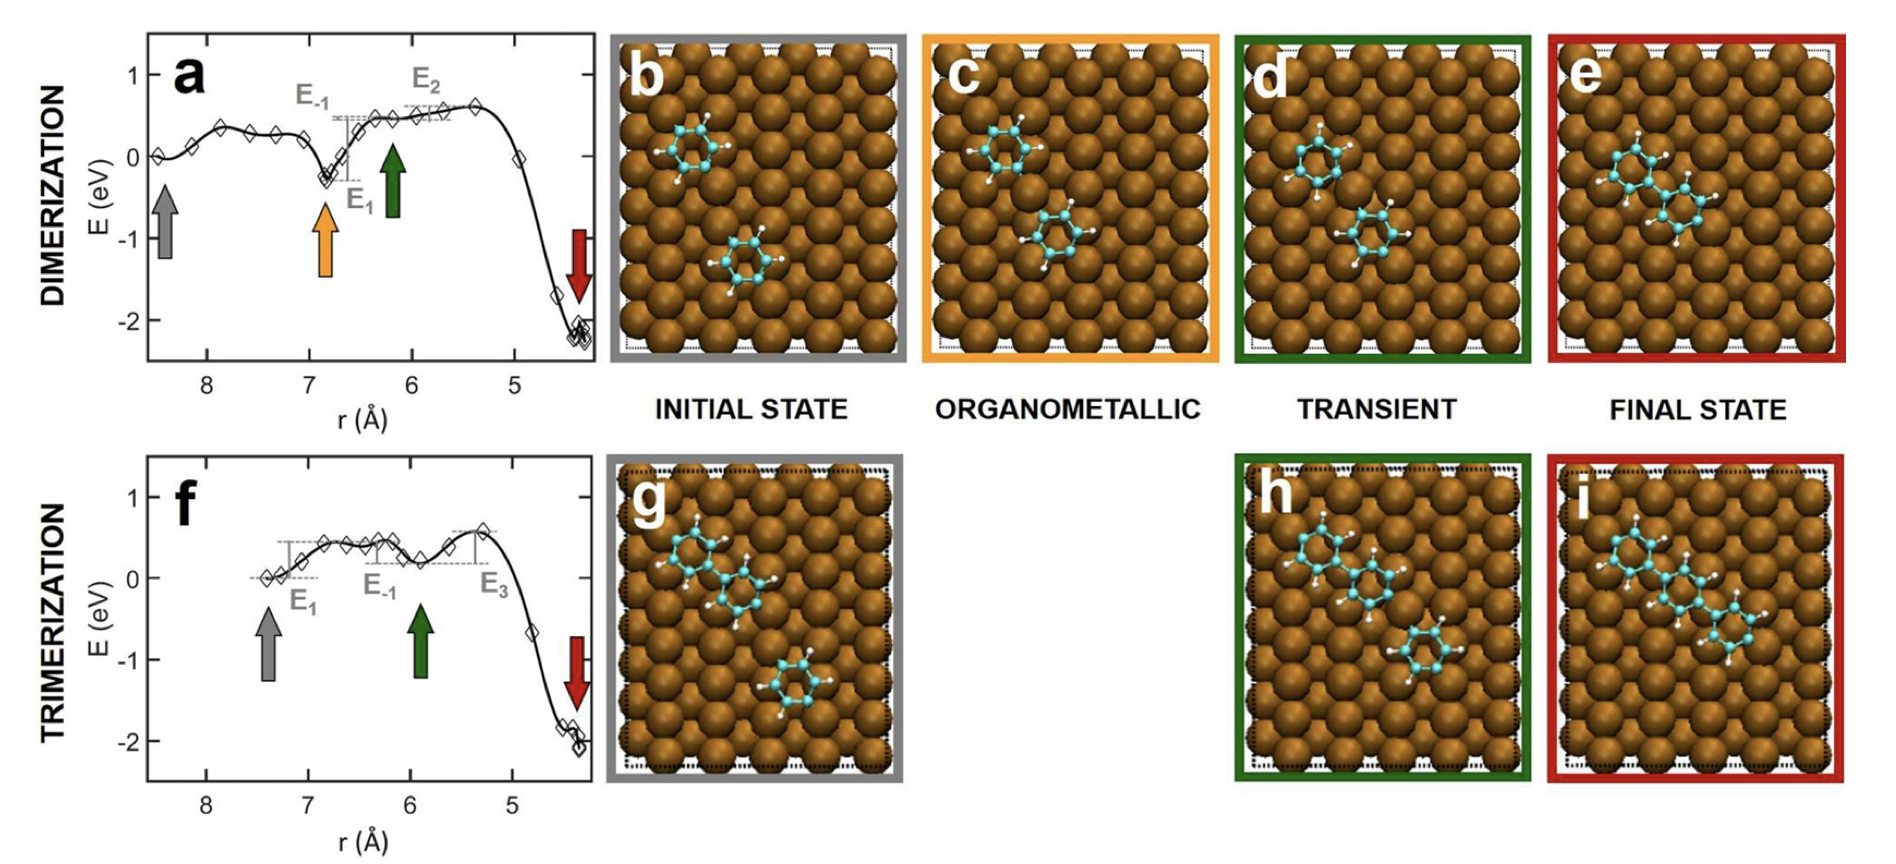
\includegraphics[width=1.0\textwidth]{Fig/Dimer_trimer.png}
%R1111: What metal is this. Better captions are required for all figures. Chemical identity of all species must be clear from the figure.
%\caption{Coupling barriers between (a) two monomers (dimerization) and (f) a monomer and a dimer (trimerization), respectively. The length (r) indicated in angstrom is the distance between the centers of the aromatic rings which undergo covalent coupling. The geometries of the most significant states (initial, organometallic intermediate, transient, and final) are reported in panels b--e and panels g--i for the dimerization and trimerization, respectively. The colors of the frames correspond to the arrows in panels a and f.}
%\label{fig:dimer}
%\end{figure*}
%

The general trend [RZK0122: is it really true for all metals?] is that the final C--C bond formation step requires the highest temperature among all other steps of the coupling process~\cite{Naturenano2007, ullmann_70, ullmann_71}. For example, for dichlorobenzene, dibromobenzene and diiodobenzene on Cu(110), the formation of C--C bond requires a temperature ranging from \SIrange{410}{450}{\kelvin}, which is noticeably higher than the \SIrange{170}{370}{\kelvin} temperature needed for the dehalogenation~\cite{ullmann_44}. 
RZK0122: The following sentence is inconsistent with the previous section.
On other type of Cu surface, as well on Ag and on Au surface, a higher annealing temperature for C--C coupling has also been
reported than dehalogenation steps~\cite{Naturenano2007, ullmann_70, ullmann_71}.

{\color{blue}

RZK0122: The following sentence is also inconsistent with the previous section. It should be explained and placed in the next section, where all steps analyzed together.  
Comparative analysis of different metal surfaces shows that the C--C bond formation requires \SIrange{330}{420}{\kelvin} temperature on Ag surface and \SIrange{500}{600}{\kelvin} on Au surface~\cite{ullmann_51}. On Cu, the temperature range is usually lower than on Au but higher than on Ag. This indicates that the energy barrier of the formation of C--C bond step on the three metal surfaces should follow Au $>$ Cu $>$ Ag. 
}

%RZK0122: The same analysis from the bond strength perspective could be useful. Ignore this comment for now.

\subsubsection{Summary on mechanism of surface Ullmann Coupling}

{\lock

The effect of halogens and metals on each step of the surface Ullmann coupling reaction mechanism has been investigated both experimentally and computationally. 

} %lock

RZK0122: Fig.~\ref{fig:temp} is a very useful figure. We need to create our own for phenyl groups: 3 halogens and 3 metals.

\begin{figure}[ht]
\centering
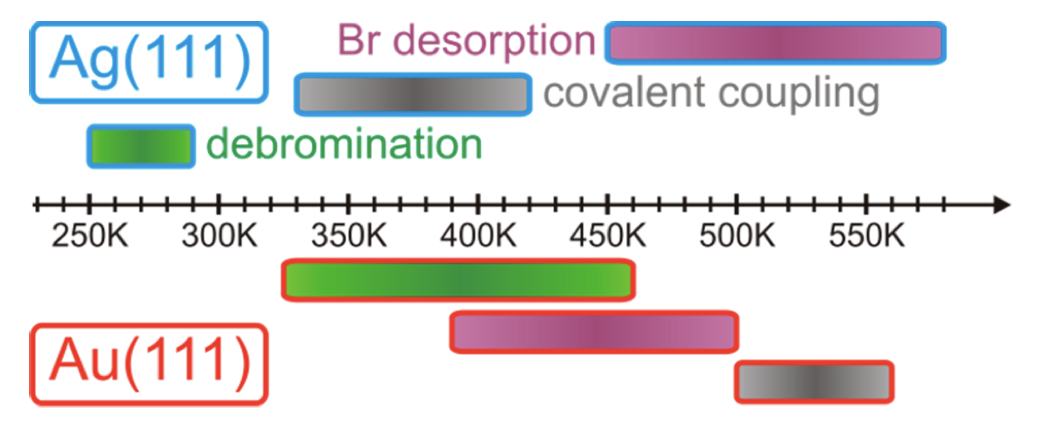
\includegraphics[width=0.75\columnwidth]{Fig/steptemp.png}
\caption{Overview and Comparison of the Temperature Ranges for Debromination (Green), Covalent Coupling (Gray), and Thermal Desorption of Bromine (Violet) on Ag(111) (Top) versus Au(111) (Bottom) As Deduced from Both Br 3d and C 1s TP-XPS Data}
\label{fig:temp}
\end{figure}

{\lock

%RZK0122: The idea and references are taken from jacs2016. Check Cu(111) trend.
The onset temperatures of the dehalogenation and C--C bond formation steps are ultimately determined by the surface reactivity. Since carbon-metal steps are formed during the first step and broken during the second step the energy barriers for these two steps are often anticorrelated~\cite{jacs2016:34}. On surfaces such as Au(111) where the dehalogenation barrier is high the barrier for ejecting the metal atom from the organometallic bridge structure is often so low that the bridge state is rarely detected. In contrast, on surfaces such as Cu(110) [and Cu(111)?] where the dehalogenation barrier is low, high temperature is required to convert the intermediate states into dimers, oligomers or polymers.

}

RZK0122: Do not reiterate what you said for each step. Any other correlations between observed trends to describe? Describe any general remarks here. For example, what problems that can be resolved by learning the mechanism (e.g. well-ordered polymers for devices)?

RZK1220: What comes next is not relevant to diffusion. Should we even discuss it in the summary of the mechanism? Should we perhaps create a separate subsection "Desorption"?

Besides, as we mentioned in the diffusion section that the energy barrier for halogens to diffuse on all metal surfaces are very low, which means halogens may have a high mobility after dissociation. Although halogens are free to move, they possess a relatively high binding energy to metals. The lowest binding energy is halogens on Au(111), around \SI{2.8}{\electronvolt} and the highest is on Cu(111), around \SI{3.1}{\electronvolt}, which indicates that the halogens are even harder to desorb than those dehalogenated phenyl groups. Research also showed that the halogens remained on metal surface will further hinder the diffusion, coupling and polymerization of all kinds of phenyl species~\cite{ullmann_64,ullmann_65}. Removing the byproducts of on-surface Ullmann coupling is also of great significance.

\subsection{Role of adatoms in the surface Ullmann coupling} 

{\lock

Metal surfaces are not perfect well-ordered structures. There exists various defects on metal surfaces ranging from three-dimensional defect such as pores~\cite{ullmann_72} and cracks~\cite{ullmann_73} to planar defects such as twin boundaries~\cite{ullmann_74} and stacking faults~\cite{ullmann_75}, line defects such as dislocations~\cite{Ullmann_76} and to point defects such as adatoms~\cite{Ullmann_77} and vacancies~\cite{ullmann_78}. A variety of surface defects are shown schematically in Fig.~\ref{cyrstal_surface}~\cite{ullmann_49}.

In the process of Ullmann coupling, reactants, intermediates and final products interact directly with metal atoms on the surface and, therefore, are affected by surface defects. Quantifying the extent to which imperfections of the metal surface influence the thermodynamics and kinetics of the Ullmann coupling can suggest new strategies for surface optimization, leading, in turn, to higher yields of desirable perfectly-assembled two-dimensional polymers. 

\begin{figure}[htb]
\centering
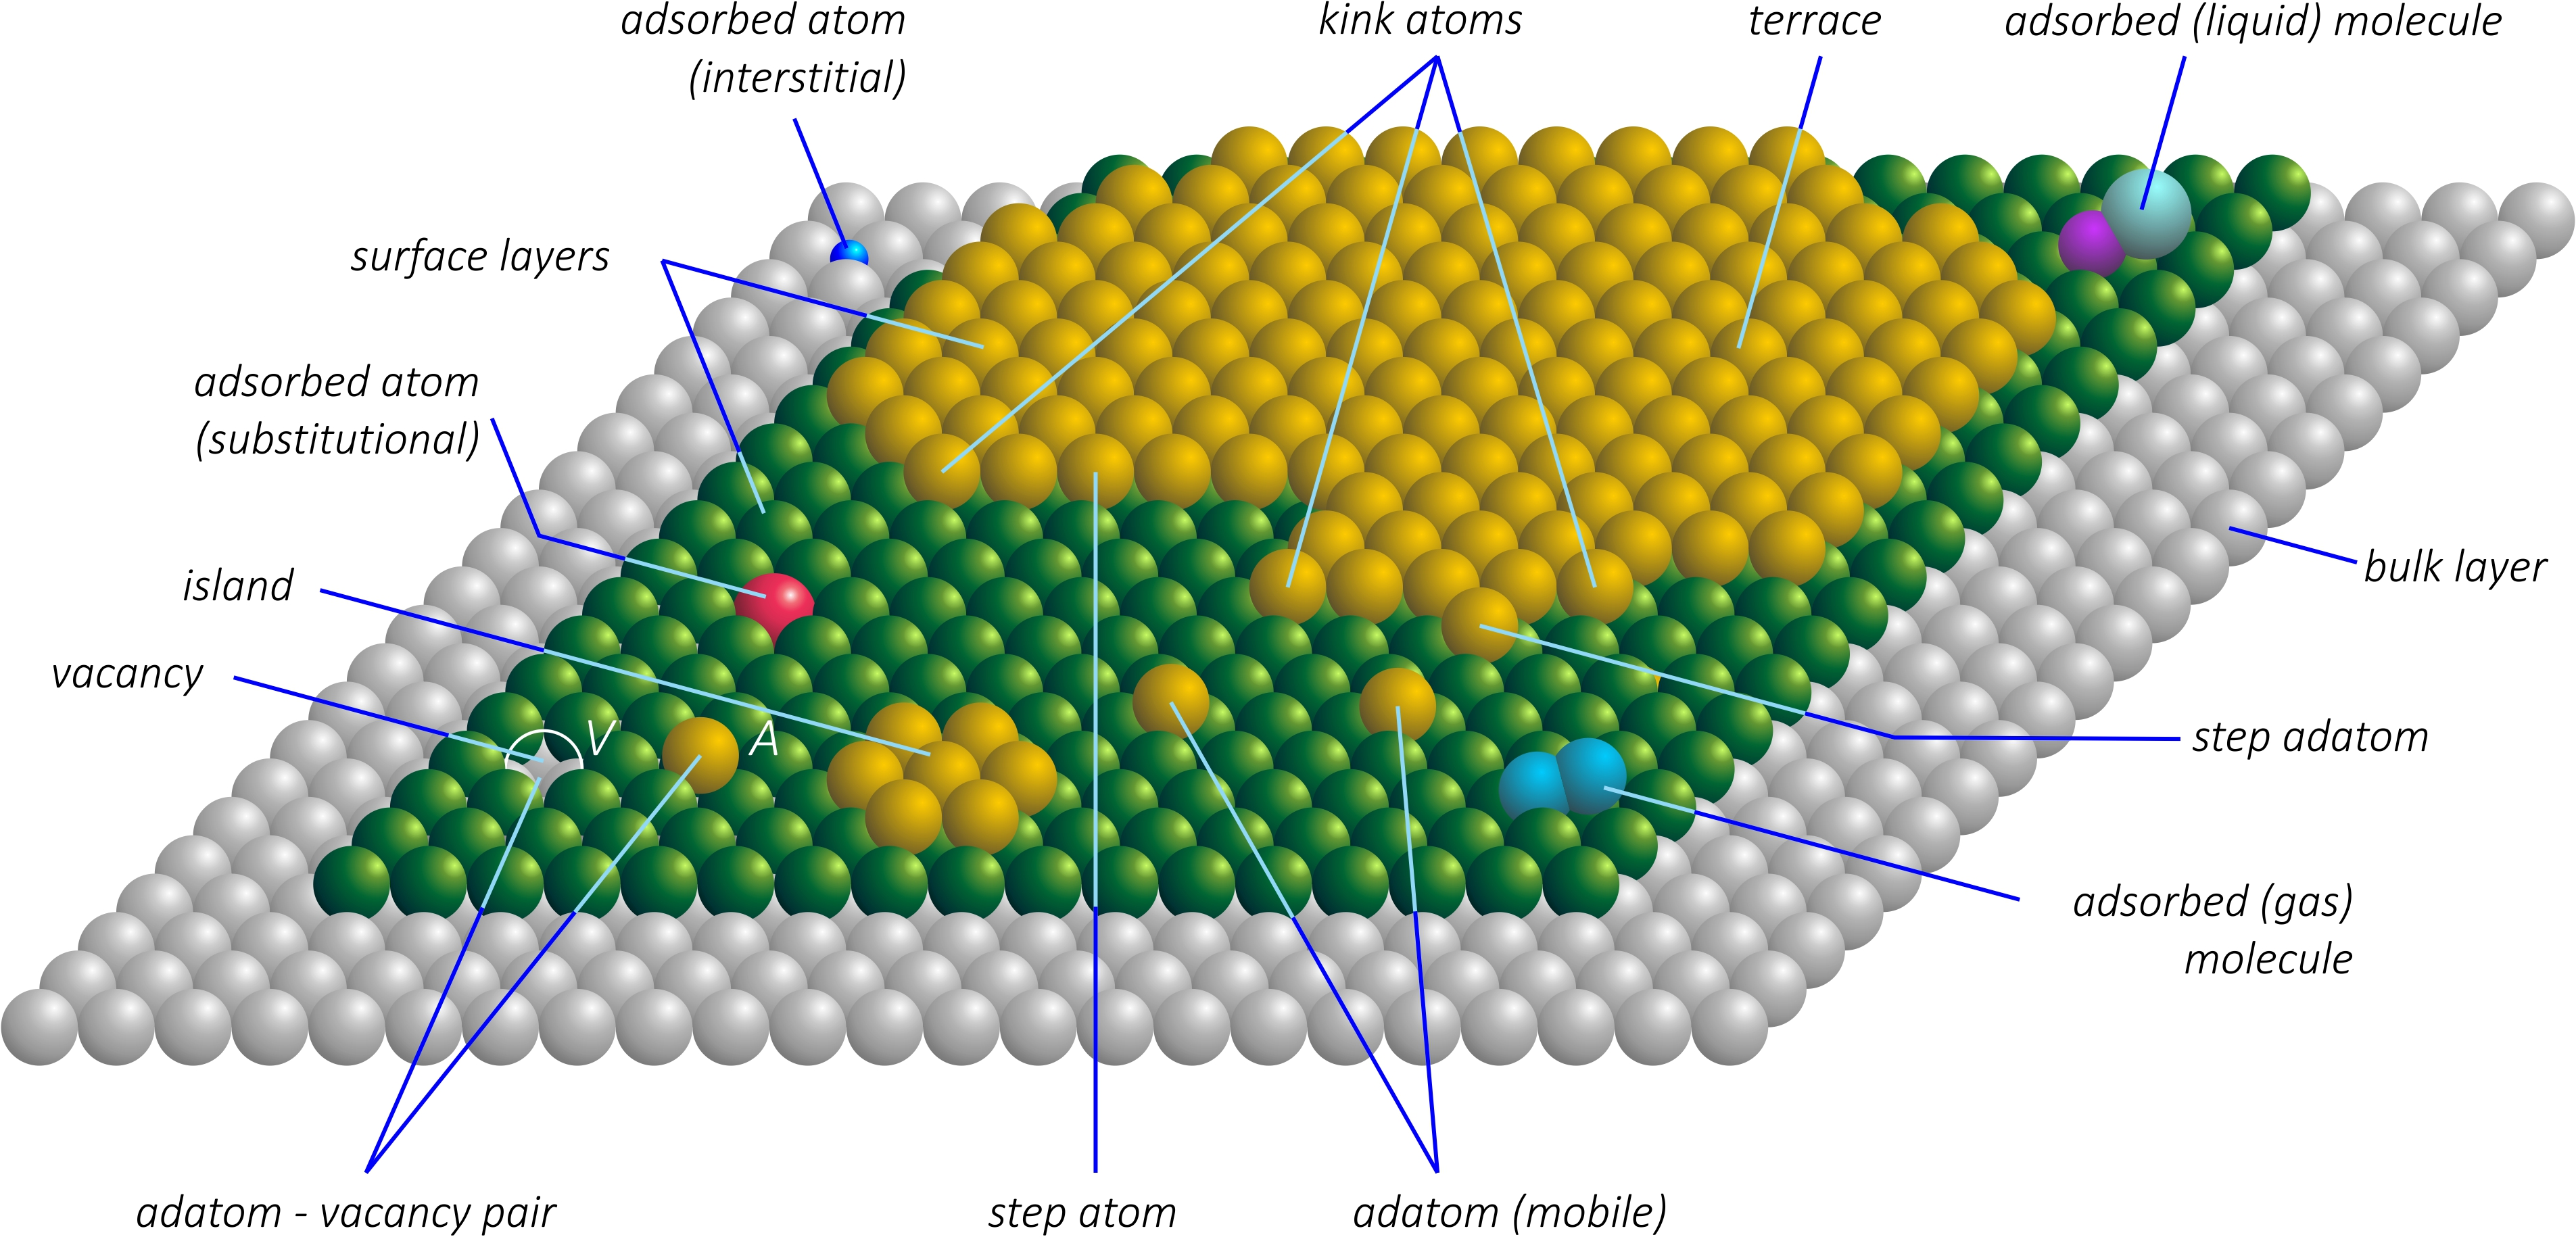
\includegraphics[width=0.4\textwidth]{Fig/Crystal_surface.jpg}
\caption{A model of crystal surface. Adapted from Ref.~\onlinecite{ullmann_49}.}
%RZK1221: Ignore at the moment. Remove the figure or find/create better figure. The text is almost invisible in this figure. 
\label{cyrstal_surface}
\end{figure}

%RZK1221: The idea to use origin(x) and nature(y) notation is inacceptable. I have never seen anyone doing this in the literature. It makes your text unreadable -- readers will have hard time remembering what your numbers stand for. Go over your text and replace all instances with simple phrases describing your metal atoms.
%nature(1) = ideal-surface atom
%nature(2) = adatom
%origin(1) = pre-existing adatom
%origin(2) = extracted adatom

Surface metal atoms that affect and participate in the Ullmann coupling have different \emph{nature} and \emph{origins}.
Atom's nature describes its immediate environment. Atoms located in the first layer of atoms of the ideal surface will be referred to as \emph{ideal-surface} atoms. \emph{Adatoms}, according to the commonly accepted definition, lie on top of the layer of ideal-surface atoms. In this work, adatoms are differentiated according to their \emph{origin} and can be \emph{pre-existing} and \emph{extracted} adatoms. The origin of pre-existing atoms is irrelevant, not specified, or not known. Extracted adatoms, on the other hand, are known to have been lifted from their lattice sites and placed on top of the surface leaving a surface vacancy behind. In this work, \emph{vacancy} refers exclusively to vacant lattice positions on the surface, not in the bulk.
%RZZK: This section might be better placed into Definitions/Notation part of the manuscript.
%RZZK: The talk about nature and origins is perhaps too formalized. I will simplify it later later.

%%%Here the two terminology $Nature$ and $Origin$ will be used to distinguish the metal atoms which participate in suface Ullmann coupling.
%%%The $Nature$ of metal atoms means metal atoms can come from (1) surface atom which is located at the first layer on metal surface, is indistinguishable from other surface atoms and has no relation with surface defect, or (2) adatoms which is related to the surface defect, it will lie above the first layer of metal surface and free to diffuse.
%%%Thus, the $nature$ mainly divide the metal atoms from a surface into two categories, the first kind is indistinguishable and locate in the lattice of metal crystal, while the second kind is adatoms, which is a production of common non-order defect appeared on metal surface. 
%%%The process that gives birth to $nature(2)$, adatoms in surface Ullmann coupling reaction is also of great interest. It can be split into two different kinds with notation $origin$: adatoms in surface Ullmann coupling may come from (1) pre-exsiting adatoms before the occurrence of surface Ullmann coupling due to the surface defect, thermal punctuation or (2)pulled out by the intermediates produced in surface Ullmann coupling, and then fully sit above the first layer of metal surface to become a new adatom. For the second origin of adatoms, it can also be expressed that the surface Ullmann coupling create this adatom which used to be a $nature(1)$ atom. 

} %lock


{\color{blue}

The nature of metal atoms and the origin of adatoms have been explored experimentally and computationally.
%For origin(1), it has been reported that the onset of the vacancy-adatom formation take place on Cu(111) surface was around 900 K by molecular dynamics~\cite{ullmann_50} , which is much higher than the temperature required by surface Ullmann coupling reaction, as shown in Fig.~\ref{fig:2Dgasn}~\cite{ullmann_50}. This could be the evidence that there would not be new adatoms formation due to the thermal fluctuations as the surface Ullmann coupling proceeds. 

%discuss that adatoms could exit on metal surface due to the thermal evaporation
For \emph{pre-existing} adatoms, it has been explored that Cu adatoms can be released on Cu(111) surface by thermal activation~\cite{ullmann_79, ullmann_58}, silver and gold adatoms can be released on silver and gold surface respectively as well~\cite{ullmann_84, ullmann_85}, especially near surface defects. These adatoms have also been previously observed to
participate in metal organic coordination networks~\cite{ullmann_80, ullmann_81, ullmann_82, ullmann_83}. This coordination phenomena provides a feasible 
possibility that the formation of carbon--metal intermediates in surface Ullmann coupling can directly make use of \emph{pre-existing} adatoms.
Thus, it can be naturally derived that there is a competition between \emph{ideal-surface} atoms and \emph{adatoms} which actually take part in the structure of intermediates in Ullmann coupling. Also if it is \emph{ideal-surface} atoms that comprise intermediates, these \emph{ideal-surface} atoms can also be fully extracted out from the first layer and become \emph{extracted adatoms}, which can be regarded as an approach to create adatoms on metal surface.
The details of the these arguments are discussed in following sections.

%\begin{figure}[ht]
%\centering
%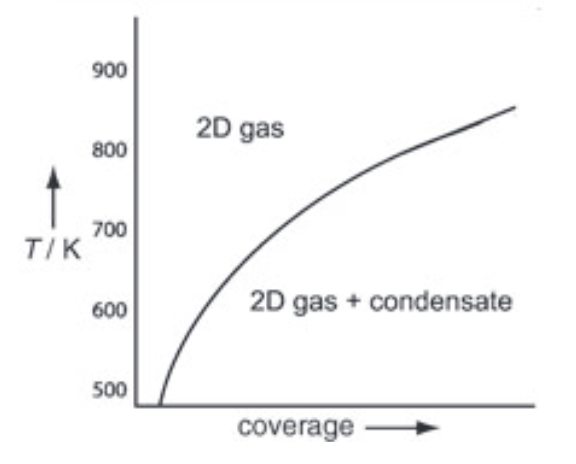
\includegraphics[width=0.75\columnwidth]{Fig/2D-gas.png}
%\caption{Schematic diagram of 2D adatom gas phase and condensed phase (islands) %coexisting at elevated temperatures for metal-on-metal systems.}
%\label{fig:2Dgas}
%\end{figure}


}

\subsubsection{Dehalogenation}

\begin{figure}[htb]
\centering
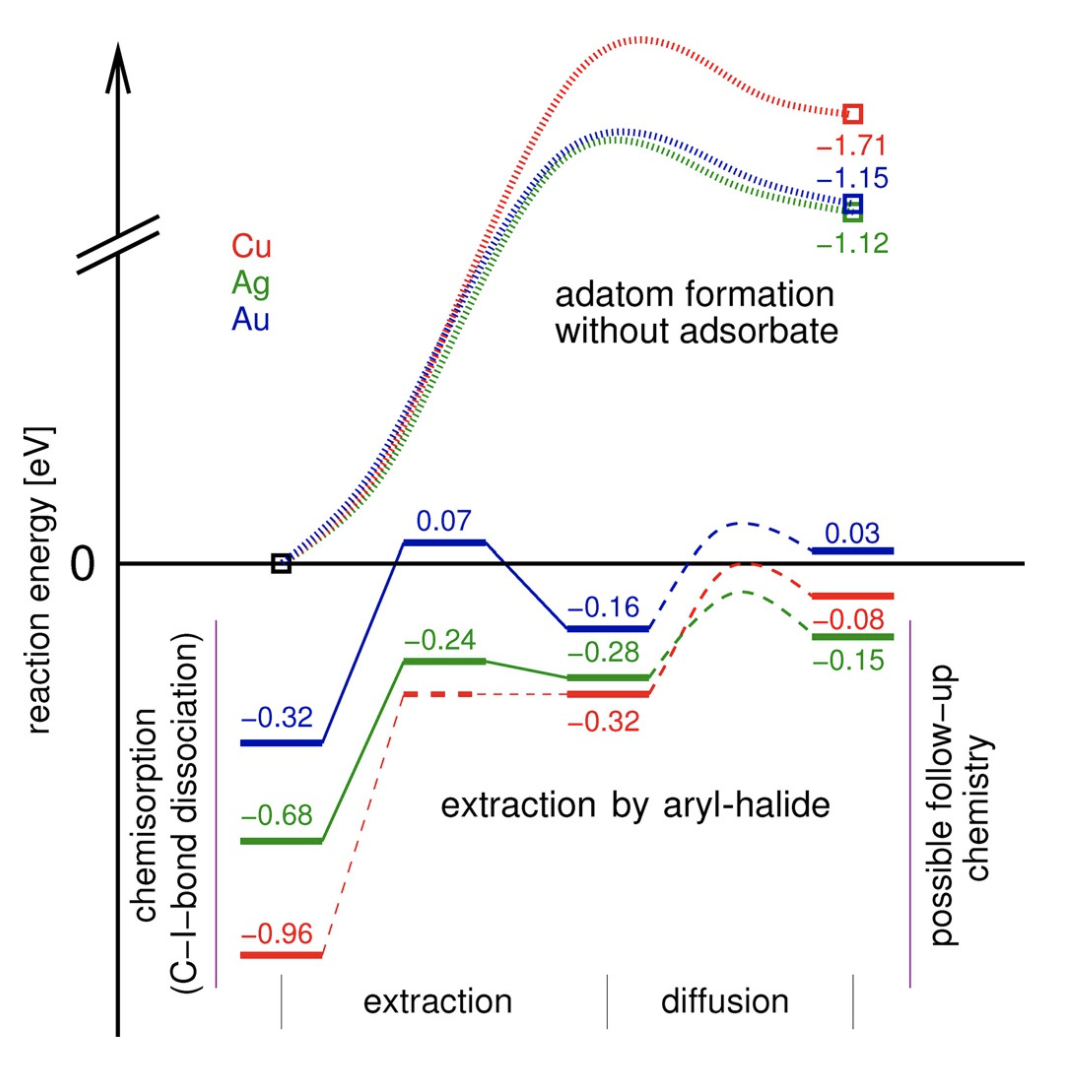
\includegraphics[width=0.75\columnwidth]{Fig/Adatom-formation.png}
\caption{Graphical comparison of the energetics of the adatom formation without adsorbate (top half) to the extraction by aryl–halide process (lower half).Values for Cu are shown in red, for Ag in green and for Au in blue. The extraction-by-arylhalide process starts from the dissociated iodobenzene. Dotted lines indicate parts of the energy profile that have not been quantitatively resolved.}
\label{fig:3}
\end{figure}

{\color{blue}

A multitude of evidences have been presented that metal atoms will participate in dehalogenation as discussed in above section. However, it is still unclear whether \emph{ideal-surface} atoms or \emph{adatoms} are involved in this process. DFT calculations demonstrated that dehalogenation, as the first step of Ullmann coupling, has possibility to originate an absolute new adatom by fully extracting an \emph{ideal-surface} atom out from the first layer~\cite{chemeurope2017}. As shown in Fig.~\ref{fig:3}, formation of an adatom on ideal, perfect Cu(111), Ag(111) and Au(111) surface require \SI{1.71}{\electronvolt}, \SI{1.12}{\electronvolt} and \SI{1.15}{\electronvolt} respectively. Dehalogenation of iodobenzene will result in phenyl-metal species, this interaction will decrease the full extraction of \emph{ideal-surface} atom by \SI{1.07}{\electronvolt}, \SI{0.72}{\electronvolt} and \SI{0.99}{\electronvolt} on Cu(111), Ag(111) and Au(111) surface, respectively. The significant reduction in energy indicates that a new adatom can probably be created from an \emph{ideal-surface} atom by organometallic intermediates produced in dehalogenation. 

But it has also been reported that the interaction between single phenyl groups and copper atoms are not adequate enough to fully extract an \emph{ideal-surface} atom out. These phenyl groups produced after dehalogenation will start to diffuse on Cu(111) surface and interact with different \emph{ideal-surface} atoms to form organometallic intermediates~\cite{pccp2010} while all \emph{ideal-surface} atoms involved will stay on their original locations after diffusion.

Till now it can be concluded that dehalogenation lowers the energy required for creation of adatoms from \emph{ideal-surface} atoms on a metal surface. The direct use of \emph{pre-existing} adatoms should ideally cut down the energy needed for this step compared to \emph{ideal-surface} atoms. However, few work has been related to \emph{pre-existing} adatoms in dehalogenation.

}

%Evidences have already been presented that metal adatoms participate in the process of dehalogenation. 
%In 2017, Barton \textit{et al.}~\cite{chemeurope2017} explored the role of adatoms in the dehalogenation step with iodobenzene on Au(111), Ag(111) and Cu(111) surface based on DFT calculations. The energy profile of adatom formation on pristine surface was compared with the profile of formation on surface with the presence of iodobenzene, the latter case is referred to as adatom formation of $origin(2)$. The comparison has shown that the energy of extracting a metal atom from the pristine surface was in the 1.12 - 1.71~eV range. While in the dehalogenation step, the dehalogenated iodobenzene would interact with the metal atom of $nature(1)$ on metal surface, which would possibly form a new adatom of $origin(2)$. This step required a dramatically lower energy of 0.16-0.60~eV range. Furthermore, the calculations have shown that the energy released in the process of adsorption of idobenzene on metal surface and formation of organometallic intermediates in the process of surface Ullmann coupling is sufficient to compensate the energy required for a metal atom extraction to form a new adatom of $origin(2)$, as shown in Fig.~\ref{fig:3}.
%
%It is clear that metal atoms of $nature(1)$ have a great chance to participate in dehalogenation, the first step of surface Ullmann coupling. And the construction of organometallic intermediate in the dehalogenation could possibly be a feasible pathway to form adatom of $origin(2)$. Metal atoms of $nature(2)$ in the dehalogenation had few related reports to date.


\subsubsection{Diffusion}

\begin{figure}[hbt]
\centering
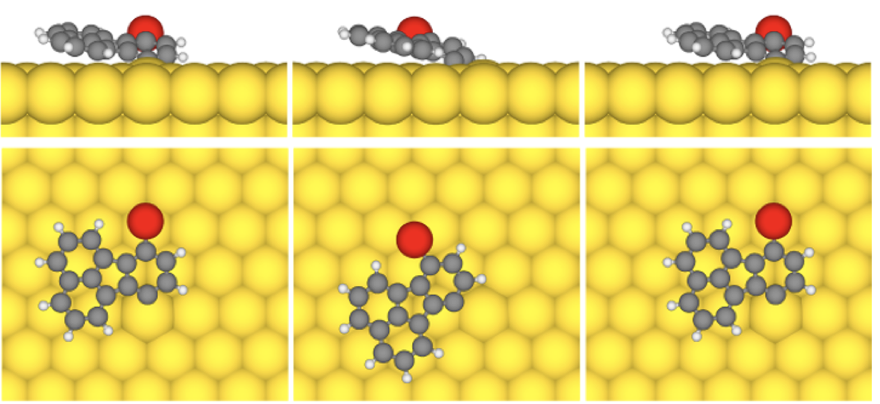
\includegraphics[width=0.75\columnwidth]{Fig/Diffusion_path.png}
\caption{Top and side view of the initial, transition and final geometries of BrFL molecule diffuse.}
\label{fig:diff}
\end{figure}

%The diffusion process is involved in the interaction between single precursor group and metal atom. 
%In 2018, Nagoya \textit{et al.}~\cite{jpcc2018} investigated the mechanism of Ullmann coupling of 7,10-dibromofluoranthene (Br$_{2}$FL) on Au(111) via DFT calculations. Compared to simple phenyl rings that tend to form ~$36^\circ$ tilt angle with Cu(111) surface~\cite{pccp2010}, the monobromo FL with one Br atom removed would stay almost parallel to Au(111) surface due to steric repulsion between the large backbone of BrFL group and the substrate. And BrFL group was found to lift surface Au atom out by 1.9 \AA\ from its initial position, which is much larger than 0.16 \AA\ height lifted by a simpole phenyl ring, as shown in Fig.~\ref{fig:diff}.
%Ebeling \textit{et al.}~\cite{acsnano2019} also indicated 4-bromo-3$^{''}$-iodo-$p$-terphenyl group interacts with the Cu atom inside the surface, and would partially lift the Cu atom out from the surface while diffusing on Cu(111) surface. 
%
%Metal atoms of $nature(1)$ were proven to play a significant role in the diffusion of dehalogenated phenyl groups, the metal atoms that interact with phenly groups will be partially lifted from its original position, the lifting height is affected by the intensity of interaction between the phenyl group and metal atom. Formation of adatom of $origin(2)$ has not been reported in diffusion, which indicates that the interaction between phenyl group and metal atom in this step is not in the magnitude to fully extract a metal atom of $nature(1)$. 

{\color{blue}

There were no apparent proof that diffusion of dehalogenated species on metal surface can form new adatoms from \emph{ideal-surface} atoms. Most reports were focused on the interaction between the dehalogenated intermediates with \emph{ideal-surface} atoms in diffusion process. The magnitude of this type of interaction is determined by the geometry of intermediates and type of metal atoms.

For single phenyl groups diffusing on Cu(111), it will form \SI{36}{\degree} tile angle with respect to the surface, and the ring structure will flip when it moves between two adjacent copper atoms. Phenly group will lift the \emph{ideal-surface} copper atom by \SI{0.16}{\angstrom} from its original position in diffusion~\cite{pccp2010}. When it comes to the bromofluoranthene molecule diffuse on Au(111) surface, DFT calculation reveals that this aryl group will stay almost parallel to the surface~\cite{jpcc2018}. And the \emph{ideal-surface} gold atom will raise up to \SI{1.9}{\angstrom} from the first layer, \SI{1.74}{\angstrom} higher than phenyl-cooper, owing to the stronger interaction between bromofluoranthene and gold atom.

Whether \emph{pre-existing} adatoms are involved in this step is rarely reported. It can be concluded that diffusion of aryl groups on metal surface can seldom create adatoms since the intensity of interaction between these single dehalogenated species and metal atoms is not sufficient to fully extract \emph{ideal-surface} atoms out.

}

\subsubsection{Formation of C--M--C structure intermediates} \label{sec:dimerized-adatom}

%The nature of the metal atoms in dimerized organometallic intermediate has been investigated through multiple approaches. Besides, it can be deduced that an metal atom of $nature(2)$, which is also an adatom of $origin(1)$ will exit above the first layer of surface before the surface Ullmann coupling reacion occurs. And this atom can attract two phenyl groups diffuse close to it and form the dimerized organometallic intermediate in this step. This type of formation might require less energy compared to the situation that two phenyl groups both interact with the same metal atom of $nature(1)$. The arguments on the nature and origin of metal atoms in this step are intense in the mechanism of surface Ullmann coupling.

%In 2017, Zint \textit{et al.}~\cite{acsnano2017} analyzed structures of intermediates in the polymerization of bromotriphenylene to bistriphenylene on Cu(111) surface using STM, AFM image and DFT calculations. Two computational models were compared: two triphenylene molecules bonded to an fully-out-of-surface adatom (a metal atom of $nature(2)$) and two precursors bonded to an atom partially lifted from Cu surface (a metal atom of $nature(1)$) as shown in Fig.~\ref{fig:5}. It has been concluded that the structures observed in AFM were more consistent with computational adatom ($nature(2)$) models. In particular, the C--C distance in organometallic intermediate was of 3.9 \AA\ measured by AFM, which was closer to the Cu adatom ($nature(2)$) model (3.86 \AA) compared to the partially-lifted Cu atom ($nature(1)$) model (3.42 \AA). Furthermore, the energy for formation of the adatom-containing intermediate from distant precursors was 1.74~eV lower than that of the intermediate with a partially lifted atoms. 

\begin{figure}[hbt]
\centering
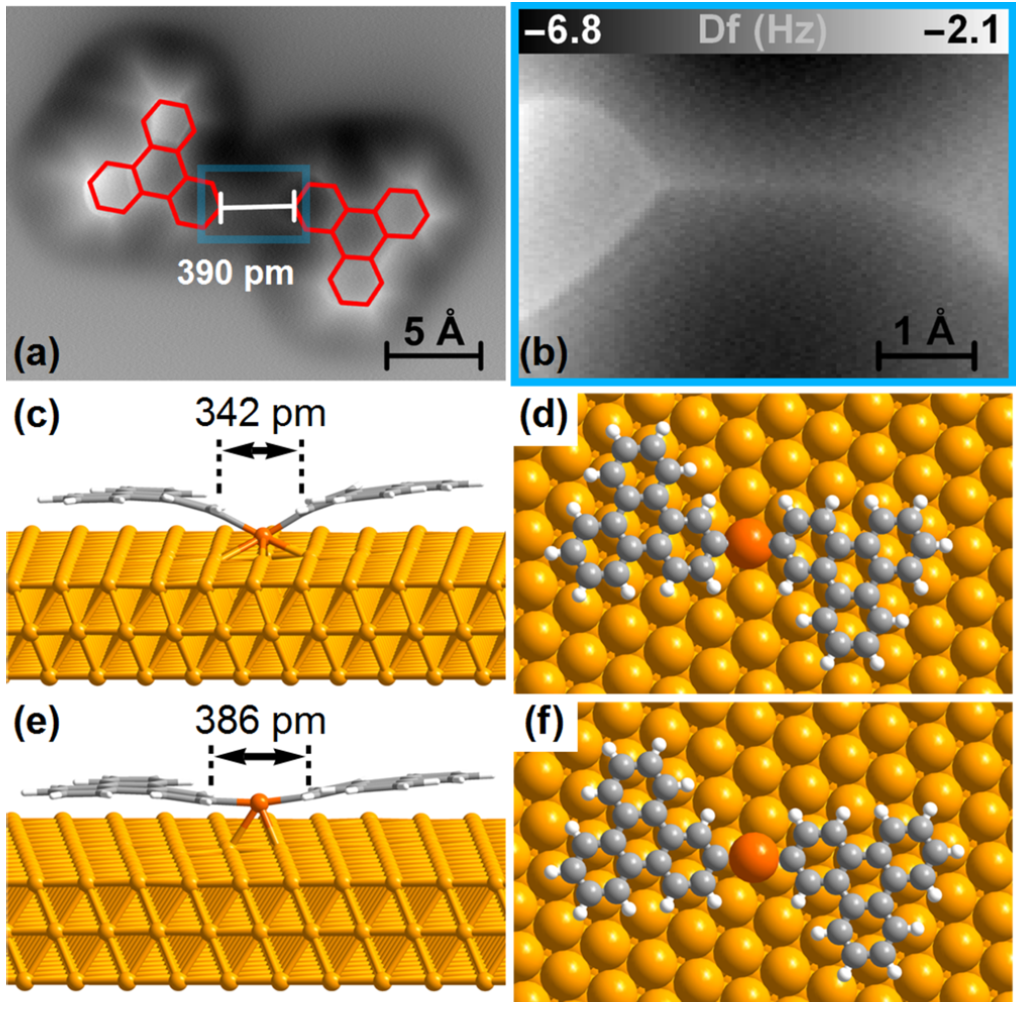
\includegraphics[width=0.75\columnwidth]{Fig/distance.png}
\caption{(a) AFM frequency shift image of intermediate with fit of structural model. (b) Zoom on intermediate bond ($cf$. blue box in a) imaged with decreased tip-sample distance ($\Delta$z = -70 pm with respect to image a). (c--f) DFT-D3 calculations [PBE-D3/ pw (PAW P)] for two different organometallic intermediate states (surface atom (c,d) vs adatom (e,f)).}
\label{fig:5}
\end{figure}

%The origin the adatoms were later explored after the metal atoms in dimerized organometallic intermediates were proven to be of $nature(2)$, which is an adatom on surface. In 2019, the study of 4‐Bromo-3$^{''}$- iodo‐$p$‐terphenyl coupling on Cu(111), proved again that the Cu atoms in dimerized organometallic intermediates were adatoms (metal atoms of $nature(2)$) compared experiments with simulated AFM image[Fig.~\ref{fig:6}~\cite{acsnano2019}]. It was further suggested that these adatoms are generated by the extraction of two close single precursor groups (adatom of $origin(2)$), instead of pre-exsiting adatoms (adatoms of $origin(1)$) from a statistic study of all intermediates species in the surface Ullmann coupling.

\begin{figure}[ht]
\centering
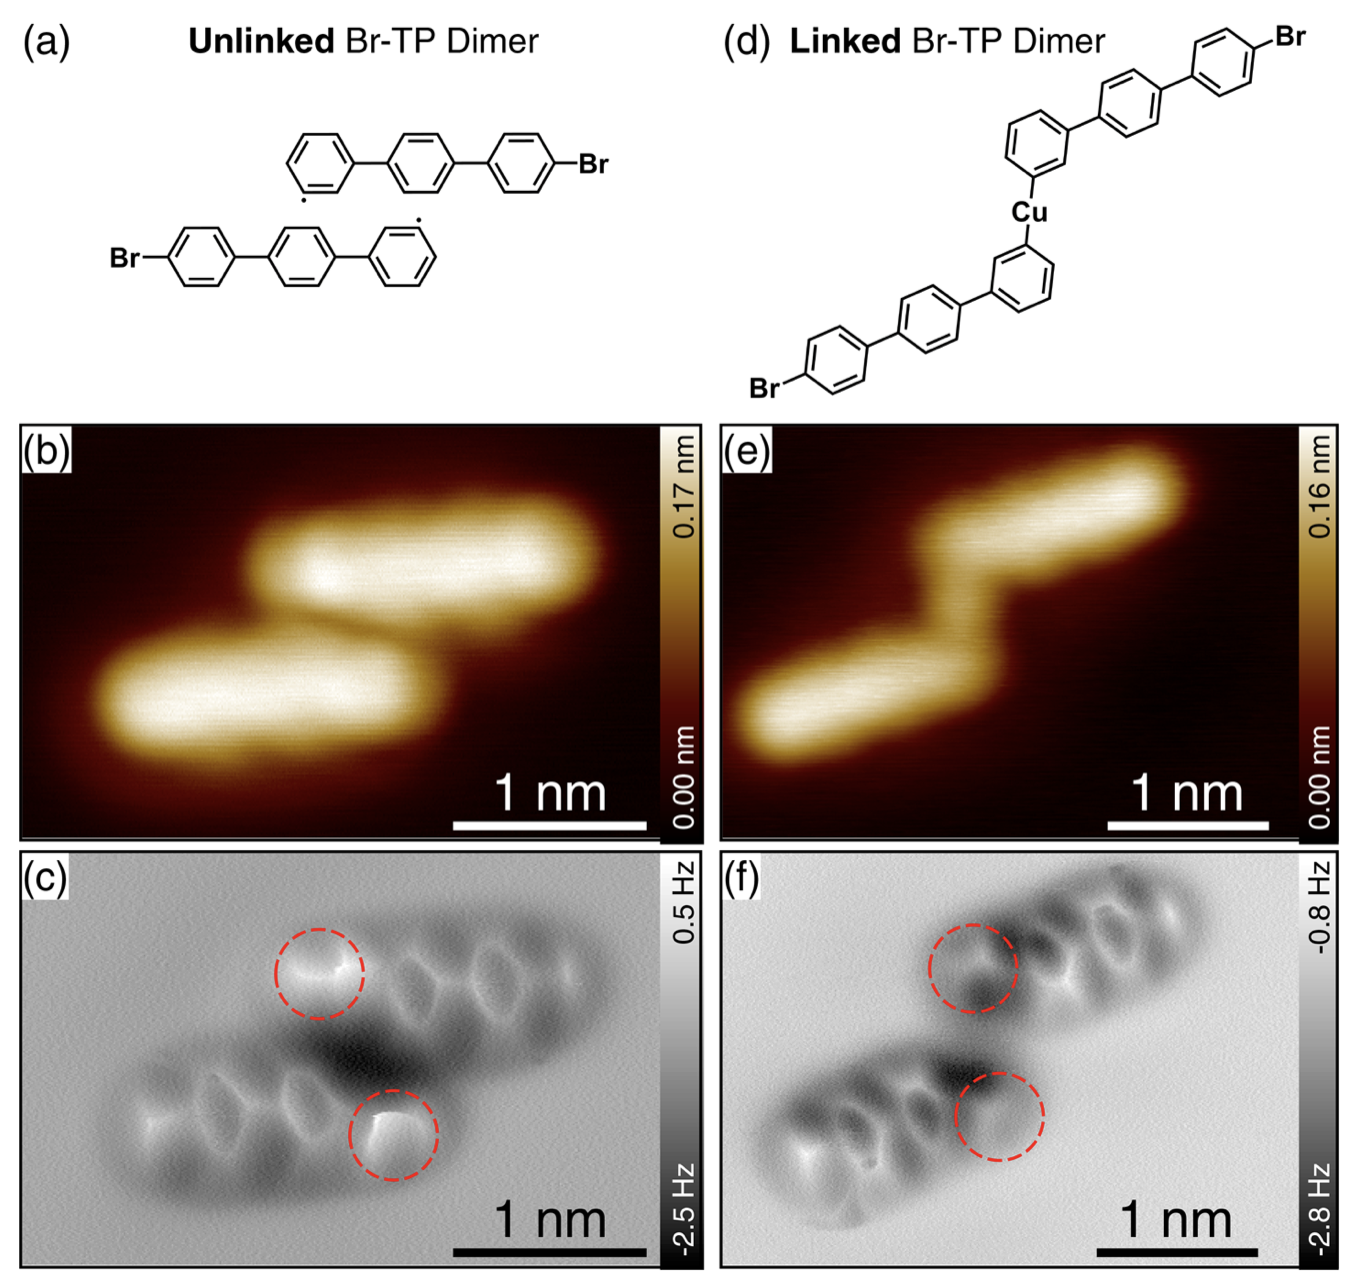
\includegraphics[width=0.75\columnwidth]{Fig/AFM_prove.png}
\caption{Molecular structures (top row), STM (middle row), and AFM images (bottom row) of 4‐Bromoterphenyl dimers on Cu(111). Two different types of dimers are observed, which are denoted as unlinked (left column) and linked dimers (right column). The STM image of the unlinked dimer reveals a dark region between the two molecules that separates them. Between the two molecules of the linked dimer a bright protrusion is observed in the STM scan that directly links them. The red dashed circles in (c) and (f) indicate the twisted phenyl rings, which lost their iodine atoms. Imaging parameters: (b) 200 mV, 30 pA, (e) 200 mV, 10 pA, tip height z = -100 pm (c) and z = -24 pm (f) with respect to a tunneling set point of 200 mV and 10 pA on Cu(111).}
\label{fig:6}
\end{figure}

%The nature of metal atoms in dimerized organometallic intermediates has been proven to be an adatom. And further the origin of this adatom is of $origin(2)$, which indicates before the surface Ullmann coupling reaction occurs, the adatom is still a metal atom of $nature(1)$, stay in the first layer of metal surface. After it was selected from two phenyl groups in coupling procedure, it will be fully lifted out of the surface, become a new adatoms. The effect of metal atom in the last step --- formation of C--C bond was not investigated intensive compared to previous steps.

%%In addition, chlorinated prophyrin as precursor has also been deposited on Cu(111)~\cite{chematerial2019}. Based on DFT calculations, the Cu adatom mediated path is 3~eV lower than the direct dechlorination. And from STM image, some precursors are still intact at temperature of 400~K, which should be already dehalogenated at lower temperature. It proves that the Cu adatoms are the limiting agent [Fig.~\ref{fig:prophyrin}].

%\begin{figure}[ht]
%\centering
%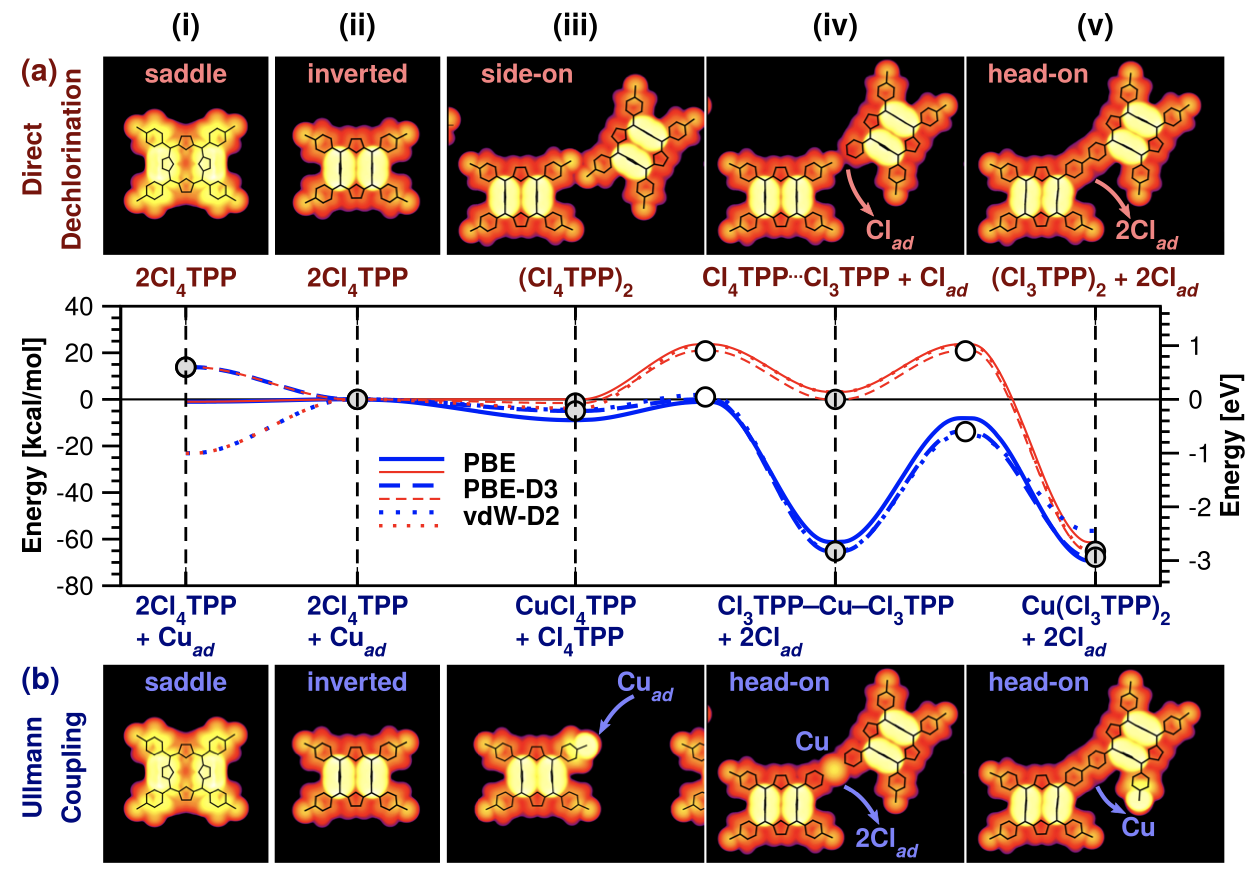
\includegraphics[width=0.4\textwidth]{Fig/Complete.png}
%\caption{STM simulations and DFT reaction profile for the (a) direct %dechlorination reaction (red lines) and (b) Cu adatom-mediated Ullmann coupling reaction (blue lines). For each process the energy are plotted of the (i, ii) precursors, (iii, iv) intermediates, (v) and final species (gray circles) and two transition states (white circles).}
%\label{fig:prophyrin}
%\end{figure}

%%ZHZH Dima suggests partial lifting should be discussed separately.
{\color{blue}
The mechanism of metal atoms participating in the formation of C--M--C bridges structure are most intensively investigated among all other steps in surface Ullmann coupling. Multiple approaches have been used to figure out it is \emph{adatoms} or \emph{ideal surface} atoms that actually constitute the C--M--C bridge. 

DFT calculation results state that two phenyl groups, after diffusing to adjacent position, will bind to the same \emph{ideal surface} copper atom and form C--Cu--C structure on Cu(111)~\cite{pccp2010}. Similar structure will be constructed on Ag(111) and Au(111) surface from phenyls and \emph{ideal surface} silver and gold atoms.

However, disagreement has been proposed with other precursors. Fig.~\ref{fig:5} describes the C--Cu--C structure formed by two triphenylene groups with a copper atom on Cu(111) surface using AFM and DFT methods~\cite{acsnano2017}. Two distinct simulation models are shown: (1) the copper atom in C--Cu--C structure comes from \emph{ideal surface} atom as shown in (c) and (d). This \emph{ideal surface} atom is partially lifted up from its original position in the first layer of metal; and (2) the copper atom in C--Cu--C is an \emph{adatom} as pictured in (e) and (f). Two model are compared with AFM image on atomic properties. The distance between carbon and carbon in this C--Cu--C bridge in AFM, \emph{ideal surface} model and \emph{adatom} model are \SI{3.90}{\angstrom}, \SI{3.42}{\angstrom} and \SI{3.86}{\angstrom} respectively, which proves that the \emph{adatom} model is more consistent with the molecule geometry in experiment. In addition, the energy required to form the C--Cu--C bridge structure from these precursors with \emph{adatom} is estimated to be \SI{1.74}{\electronvolt} lower than with \emph{ideal surface} atom. The metal atoms in C--M--C intermediate structure were proven to be adatoms with clear evidence for the first time. Then the pathway of emerging such adatoms was also reported.

In Fig.~\ref{fig:6}, the STM and simulated AFM image of forming C--Cu--C intermediate structure from 4‐bromoterphenyl and copper atom are displayed~\cite{acsnano2019}. Based on the comparison of the experimental STM and simulated AFM image data, the metal atom participated in the C--Cu--C structure is again, proven to be adatoms. Furthermore, these adatoms, according to the statistic data, are created during the surface Ullmann coupling reaction by extracting the \emph{ideal surface} atoms out instead of \emph{pre-existing} adatoms before the coupling process.

In this step, the confusion on the origin of metal atoms is approaching to be clear. Previously works suggest that the metal atoms in C--M--C intermediate structures are most likely to be adatoms. And the formation of such a bridge structure is expected to be a feasible strategy to create adatoms on Cu(111) surface. However, as discussed in former section, the intensity of interaction between aryl groups and metal atoms will be determined both by the molecule geometry of aryl group as well as the type of metal atoms. Whether surface Ullmann coupling of all possible precursors on different surfaces will obey the same mechanism still remains adequate space for further exploration and discussion.

}

\subsubsection{Formation of the C--C bond}

The  effect of adatoms on  the  formation of C--C bonds  has not been investigated as widely as on the previous steps.

\subsection{Objectives}

{\lock
%RZK1223 I will write this one.

The focus of this work is on the role of adatoms in the surface Ullmann reaction, exemplified by the coupling of two phenyl rings -- one of the most studied and simple model of the Ullmann process.

%RZZK: Further limitations of this article.
Limitation: Cu(111) only? Three halogens.

%RZZK: as well as the microscopic mechanisms of interaction of all species with various defects, energy profile

}


\section{Methods}
%\subsection{Computation Models}

\subsection{Computational Details}

%RZK: learn how to use si package and correct all units here.
The periodic density functional theory calculations were performed using the Perdew–Burke-Ernzerhof (PBE) for the exchange-correlation functional, the projector augmented wave method for the ion-core electron interactions, and a plane-wave basis set as implemented in the Vienna ab-initio simulation package (VASP) code. Van der Waals (vdW) interactions were included using the DFT-D3 method to describe the nonlocal correlation energy. 

The Cu(111) surface used in all Ullmann coupling was 
modeled by a four-layered slab consisting of 192 Cu atoms and at least \SI{15}{\AA} of vacuum. Each layer is made up with 48 ($8\times 6$) Cu atoms. The relaxations were performed with applying spin-polarization. The energy cut-off for the plane-wave basis was set to \SI{800}{\electronvolt} and a $3\times 3 \times1$ k-mesh was adopted. The mesh density of k points was kept fixed in related calculations with primitive cells. All atoms were fully relaxed until the MAX force on the atom was less than $2\times 10^{-2}$ \si{\electronvolt}/\si{\AA}$^{2}$. 

Transition-state calculations were carried out using a Climbing-Image Nudged Elastic Band (CI-NEB) methods with VTST code\cite{ullmann_59}. An improved initial guess~\cite{ullmann_60} for minimum energy path was conducted in CI-NEB calculation, different number of intermediates were interpolated between the initial and final configurations due to the distance between them. Plus, All atoms were fully relaxed until the MAX force on the atom was less than \SI{0.1}{\electronvolt}/\si{\AA}$^{2}$ in CI-NEB calculations.

Generally the value of most thermodynamic functions can be derived from our DFT optimization results. 
(%ZZ1215: still miss the math part, will add later)

The simulation of surface Ullmann coupling reaction was conducted with chlorobenzene, bromobenzene and iodobenzene on Cu(111) surface. We explored the mechanism discussed above step by step including the least reported step --- formation of C--C bond.

In the dehalogenation step, the CI-NEB method was used in chlorobenzene, bromobenzene and iodobenzene precursors to study how different halogens will affect on the dissociation of carbon-halogen bonds. CI-NEB method offered us energy profile diagram as well the transition state.

\section{Results and Discussion}

\subsection{Physisorption}

{\lock

The precursors of surface Ullmann coupling are physisorped on the Cu(111) surface before the initialization of the chemical process. The calculated adsorption energies are \SI{-1.06}{\electronvolt}, \SI{-1.18}{\electronvolt} and \SI{-1.37}{\electronvolt} for chlorobenzene, bromobenzene and iodobenzene, respectively. 
} %lock
{\color{blue}
The binding energy have been reported to be \SI{0.95}{\electronvolt}, \SI{1.12}{\electronvolt} for bromobenzene and iodobenzene on Cu(111) previously with optB86b correlation-exchange functional in DFT and a smaller slab size~\cite{jacs2013}. 
}

%RZK1223: Numbers from previous calculations. What computational methods have been used before? 


\subsection{Dehalogenation}

{\color{blue}

%RZK1223: We do not seem to need this energy at this point.
%(In the literature, they mentioned that in the gas phase, the dissociation reaction are highly endothermic (3.85 eV for bromobenzene and 3.33 eV for iodobenzene), we can get the energy for this reaction too)

Fig.~\ref{fig:dissociation_Cl}, Fig.~\ref{fig:dissociation_Br} and Fig.~\ref{fig:dissociation_I} 
%ZZ: I is under recalculation
show the initial, transition and final states (notated as IM1, TS1 and IM2 in Fig.~\ref{fig:completeenergy}) of chlorobenzene, bromobenzene and iodobenzene dehalogenation on Cu(111). The energy change ($\Delta E$ = $E_{IM2} - E_{IM1}$) and the activation energy ($E_{barrier} = E_{TS1} - E_{IM1}$) are computed, $\Delta E$ are \SI{-0.58}{\electronvolt}, \SI{-0.8}{\electronvolt} and \SI{-0.94}{\electronvolt}, $E_{barrier}$ are \SI{1.25}{\electronvolt}, \SI{0.92}{\electronvolt} and \SI{0.68}{\electronvolt} for the break of C--Cl, C--Br and C--I bond, respectively. DFT results have demonstrated that the $E_{barrier}$ of nucleophilic substitution of chlorobenzene and bromobenzene in solution are \SI{1.11}{\electronvolt} and \SI{1.18}{\electronvolt}~\cite{ullmann_86}. The discrepancy in energy indicates that the dehalogenation reaction should go through different mechanisms on Cu(111) surface and in solution. 
Contrary to on surface condition, dehalogenation of bromobenzene and iodobenzene in gas phase need \SI{3.85}{\electronvolt} and \SI{3.33}{\electronvolt} energy to accomplish~\cite{jacs2013}. This means copper surface can denote electrons to and stabilize dissociated species, which will make this reaction energetically favourable on Cu(111).  
$E_{barrier}$ of dehalogenation on surface decrease by the order C--Cl $>$ C--Br $>$ C--I. In experiment, C--I bond of iodobenzene will dissociate at \SI{175}{\kelvin}~\cite{ullmann_87}, C--Br bond of iodobenzene will be at \SI{160}{\kelvin}~\cite{ullmann_67}, and a higher temperature condition is required to break C--Cl than C--Br and C--I.
Similar procedure has also been investigated previously~\cite{jacs2013}, which offered the value for $\Delta E$ and $E_{barrier}$ of dehalogenation of bromobenzene and iodobenzene on Cu(111), $\Delta E$ are \SI{-0.70}{\electronvolt} and \SI{-0.82}{\electronvolt} and $E_{barrier}$ are \SI{0.72}{\electronvolt} and \SI{0.40}{\electronvolt} with optB86b functional and smaller slab size.

In addition the energy data, the geometry of intermediates in dehalogenation are also obtained and summarized. As shown in Figures~\ref{fig:dissociation_Cl}--\ref{fig:dissociation_I}, the distances between carbon and halogen which are going to break, the angle of phenyl ring with respect to surface are both suffering successively changes. In IM1 of chlorobenzene, bromobenzene and iodobenzene, the distance between carbon and halogen is \SI{1.74}{\AA}, \SI{1.91}{\AA} and \SI{2.12}{\AA}. These values are consistent with the calculated bond length of C--Cl (\SI{1.76}{\AA}), C--Br (\SI{1.91}{\AA}) C--I (\SI{2.14}{\AA})in gas phase based on B3LYP functional DFT calculations. C--Cl, C--Br and C--I distances have increased by \SI{0.44}{\AA}, \SI{0.55}{\AA} and \SI{0.49}{\AA} in transition state TS1 compared to the original carbon halogen bonds, respectively. Finally the dehalogenation will end in relatively stable IM2, dissociated halogen atoms occupy the hollow site on Cu(111) surface. The distance between C--Cl, C--Br and C--I increase to \SI{3.99}{\AA}, \SI{4.10}{\AA} and \SI{5.10}{\AA} in these intermediate states. The phenyl ring of chlorobenzene, bromobenzene and iodobenzene are all mostly parallel to Cu(111) surface before the dehalogenation. And in the dissociation, the phenyl rings start to become tilt on surface, and finalize at a large slope. This indicates that the carbon atoms in original carbon halogen bonds are interacting with copper atom in Cu(111) during the dehalogenation process.

Summarizing the data of the first step, Cu(111) surface has been proven to evidently reduce the energy barrier of the dehalogenation of chlorobenzene, bromobenzene and iodobenzene. The copper surface can not only serve as a template and support for Ullmann coupling reaction, but also optimize the temperature condition for it to initialize. On Cu(111), the dehalogenation of iodobenzene is the most energetically favourable and chlorobenzene is the least. The mechanisms of three different halogens dissociation are very similar according to the angles and distance change in related species.


}
%RZK: First state reaction energies. Negative energies already mean that the reaction is exothermic, there is no need to state this.

Fig.~\ref{fig:dissociation_Cl}, Fig.~\ref{fig:dissociation_Br} and Fig.~\ref{fig:dissociation_I} shows the initial, transition and final states (notated as IM1, TS1 and IM2 in Fig.~\ref{fig:completeenergy}) of chlorobenzene, bromobenzene and iodobenzene dehalogenation on Cu(111), respectively. 
Dehalogenation reactions of three precursors are all exothermic, which in reverse, are endothermic in gas phase according to the DFT calculated energies. This is due to the formation of energetically unstable radical in gas phase, but copper surface can donate electrons to stable these intermediate species.
%R1111: Do you mean our calculated enthalpies or experimental values? (%ZZ: add descriptions)
%R1111: Why your state lalbels (IM2, IM1) disagree with those in the final energy profile?(%ZZ: changed)
The energy change ($\Delta E$ = $E_{IM2} - E_{IM1}$) of dehalogenation of chlorobenzene, bromobenzene and iodobenzene on Cu(111) are -0.58 eV, -0.8 eV and -0.94 eV, respectively. As seen from the Figures~\ref{fig:dissociation_Cl}--\ref{fig:dissociation_I}, the halogens always occupy the hollow site of Cu(111) surface after the carbon-halogen bond (C-X) is broken. 
%R1111: Physisorption must be described before dissociation. Negative, not positive adsorption energies must be used
%In IM1, the precursor molecule was physisorbed by the surface, the adsorption energy are 1.06 eV, 1.18 eV and 1.37 eV, respectively for chlorobenzene, bromobenzene and iodobenzene. (%ZZ: added)
%
In the TS1, the geometry of chlorobenzene, bromobenzene and iodobenzene on Cu(111) are similar, forming a tilt angle, ready for the break of C-X, the distance of C-X are 2.18 \AA\, 2.46 \AA\ and 2.61 \AA\, respectively. 
%R1111: Report bond elongations, not only bond lengths.
After dehalogenation, the phenyl species and halogen atoms were separately chemisorbed by Cu(111) surface. In IM2, the distance between the carbon and halogen are increased by 1.81 \AA\, 1.64 \AA\ and 2.49 \AA\ compared to original distance, respectively. The geometry of IM2 for chlorobenzene, bromobenzene are similar, in which the phenyl species displayed a more tilt angle with the copper surface compared to the TS1. 
%R1111: Compare you results to Ph-I in barton2017fromation (Figure5-Cu_IS in their article). They do not have vertical position for the phenyl.  (%ZZ: recalculated, not vertical)
However, In the TS1 of iodobenzene, the phenyl specie is almost vertical to the copper surface. This makes a contribution to the highest enthalpy of iodobenzene dehalogenation. Another reason why iodobenzene possesses the highest enthalpy may come from the strongest chemisorption of Iodine on Copper. 
%R1111: Do we want to perform additional calculations to figure out the reason? Perhaps not now. (%ZZ: agree)

%R1111: The first sentence is trivial and must be removed. Do not define energy barrier in Results section. This definition is trivial and can be omitted.
Secondly, the $E_{barrier}$ ($E_{barrier} = E_{TS1} - E_{IM1}$) for three halogenation reaction were also computed and summarized, which are 1.25 eV, 0.92 eV and 0.68 eV, for C-Cl, C-Br and C-I respectively. These $E_{barrier}$ values indicate that the carbon-iodine bond is the easiest to break on Cu(111) surface while the carbon-chlorine bond is the hardest. This is consistent with the experimental data that most carbon-iodine and carbon-bromine bonds will dissociate at room temperature, but an higher temperature is required to break carbon-chlorine bonds in surface Ullmann coupling. The $\Delta E$ and $E_{barrier}$ were also computed in Björk's ~\cite{jacs2013} work. $\Delta E$ were -0.70 eV and -0.82 eV and  $E_{barrier}$ were 0.72 eV and 0.40 eVfor bromobenzene and iodobenzene on Cu(111). Trends are the same with our results, the difference between specific values may come from their use of different functional (optB86b) and the size of slab (four layers 6x6).

%R1111: Some of these findings have been reported in the literature before. Comparison to previous calculations is necessary. "Trends are the same but numbers differ. Why? Do they use the same XC functional, basis set?" (%ZZ: added)

Summarizing the dehalogenation results, the reaction mechanism of chlorobenzene, bromobenzene and iodobenzene are very comparable on Cu(111) surface, the geometry of TS1 are analogous. The phenyl species of chlorobenzene, bromobenzene form a tilt angle with Cu(111) surface and it is vertical for iodobenzene. The dehalogenation of iodobenzene is the easiest among these three reactions due to the lowest activation energy.

%R1111: All figures must be formatted to make text readable. It might be desirable to place all profiles into one figure. 
\begin{figure*}[hbt]
\centering
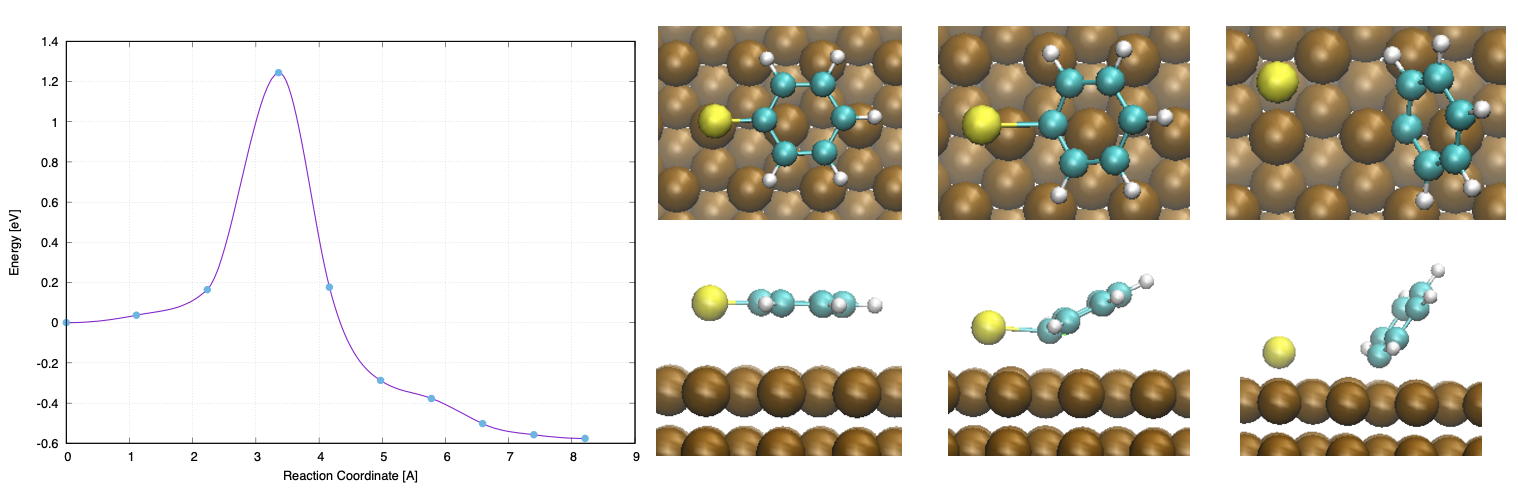
\includegraphics[width=1.0\textwidth]{Fig/dissociation_Cl.png}
\caption{The dissociation of C-Cl bond on Cu(111) surface, left is the energy diagram of the CI-NEB calculations, right side are the top and side view of $IS$, $TS$ and $FS$. (Sphere with ochre color is copper atoms, with cyan color is carbon atoms, with white color is hydrogen atoms. Same in below models. Sphere with yellow color is chlorine atom)}
\label{fig:dissociation_Cl}
\end{figure*}

\begin{figure*}[hbt]
\centering
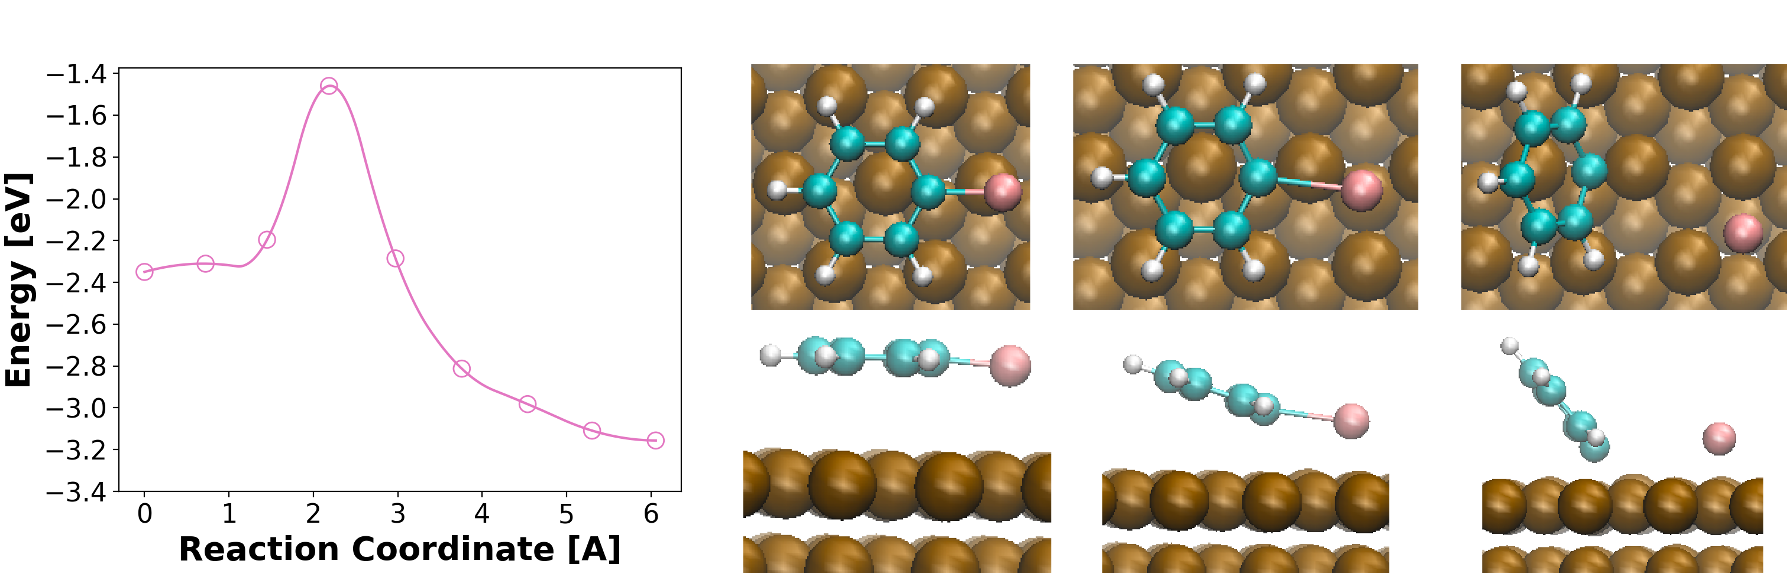
\includegraphics[width=1.0\textwidth]{Fig/dissociation_Br.png}
\caption{The dissociation of C-Br bond on Cu(111) surface. (Sphere with lime color is bromine atoms)}
\label{fig:dissociation_Br}
\end{figure*}

% \begin{figure*}[hbt]
% \centering
% 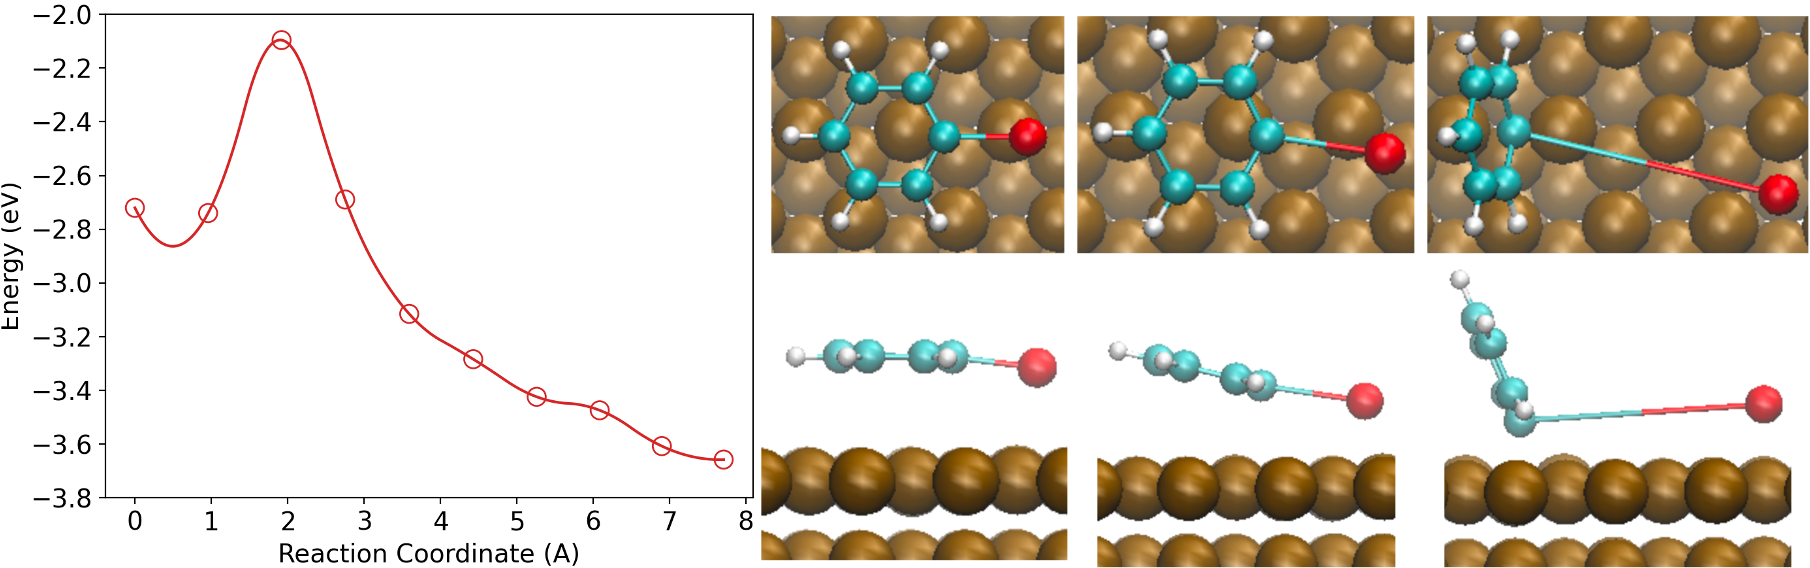
\includegraphics[width=1.0\textwidth]{Fig/dissociation_I.png}
% \caption{The dissociation of C-I bond on Cu(111) surface. (Sphere with red color is iodine atoms)}
% \label{fig:dissociation_I}
% \end{figure*}

\subsection{Formation of C--Cu--C bridge intermediates}

{\color{blue}
Fig.~\ref{fig:formingBridge} shows the energy data of forming C--Cu--C bridge intermediate structure (notated as IM4 in Fig.~\ref{fig:completeenergy}) from dehalogenated species on Cu(111) surface. $\Delta E$ of dechlorinated, debrominated and deiodinated benzene to the goose-like IM4 are \SI{0.25}{\electronvolt}, \SI{0.16}{\electronvolt} and \SI{0.17}{\electronvolt} respectively. This step for different monohalogen benzene precursors should be the same in energy after dehalogenation since the dissociated halogen atoms are not involved in this step. Our data varies slightly in chlorine, bromine and iodine, the difference comes from the approach used to obtain the energy. The initial configuration of this step is the species just finishing dehalogenation, halogen atoms are still sit close to the phenyl ring, as shown in Fig.~\ref{fig:formingBridge}. It can be speculated that there is long range interaction between the phenyl-copper intermediate and the dissociated halogen atoms. This interaction between the chlorine atom and phenyl-copper intermediate is the strongest based on the data and basically same for bromine and iodine. This initial model used here is very consistent with the experiment evidence, as in Fig.~\ref{fig:organ}, the dissociated bromine atoms all sit around in the formation of Phenyl--Cu--Phenyl structures.

In IM4 configuration, the copper interacting with two phenyl ring is initially an \emph{ideal surface} atom, and then partially lifted due to the extraction. This \emph{ideal surface} atom is raised higher by \SI{0.56}{\AA} from the first layer, while the copper atoms interact with one phenyl ring are barely extracted in IM3. It means that the force emerged between one phenyl ring and one copper atom is not adequate to extract this copper out from the surface, the strength of interaction will become sufficient when two phenyl ring diffuse to adjacent position and form such a C--Cu--C bridge structure.
The distance between two carbon atoms in C--Cu--C bridge is \SI{3.10}{\AA}, which is \SI{1.61}{\AA} longer than the bond length of single C--C bond in biphenyl. The angle of phenyl rings connected to the Cu atom with respect to the surface are both \SI{52}{\degree}, this angle is the closest to tilt angle of debrominated phenyl in IM2 (\SI{52}{\degree}), larger than dechlorinated phenyl and smaller than deiodinated phenyl.

Formation of C--Cu--C bridge structure has been proven to play a significant step in creation of adatom in surface Ullmann coupling. The interaction is potentially sufficient to extract an \emph{ideal surface} copper atom out compared to previous steps.

\begin{figure}[hbt]
\centering
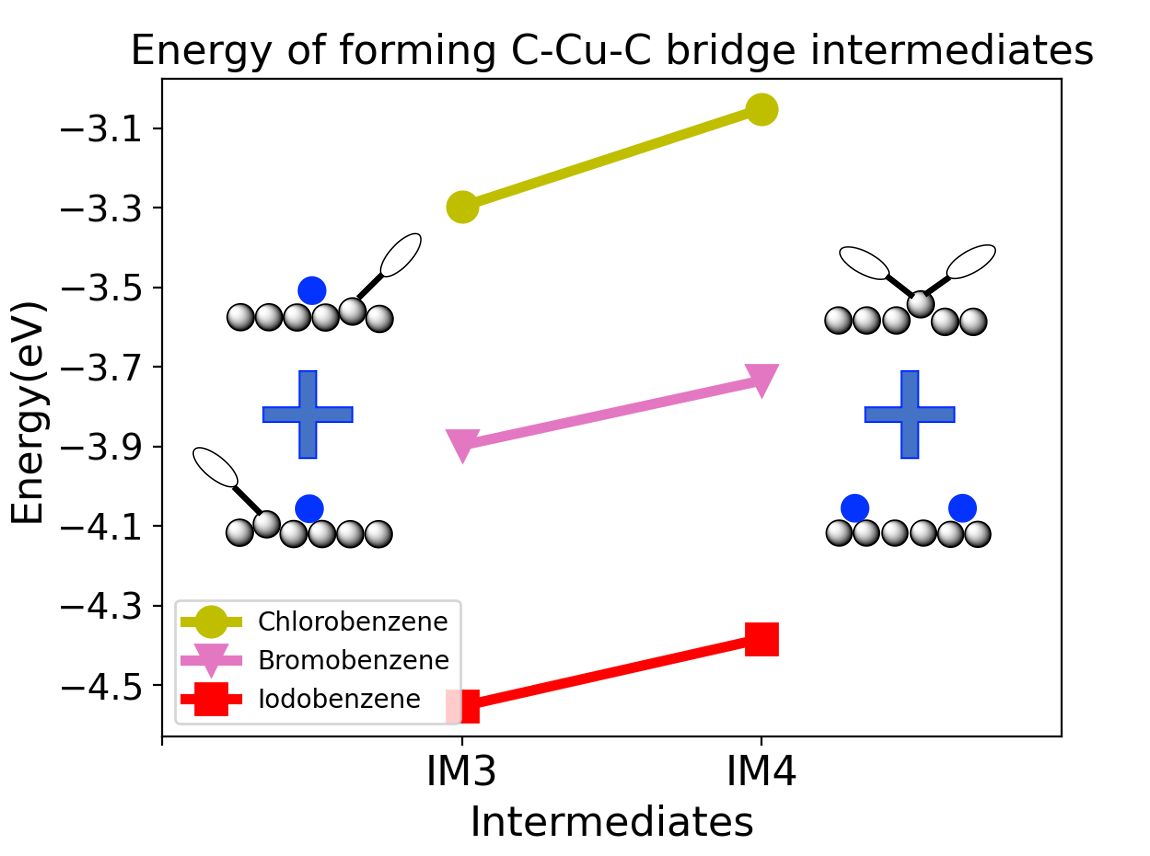
\includegraphics[width=0.45\textwidth]{Fig/FormingC-Cu-C.png}
\caption{Energy diagram of forming C--Cu--C bridge intermediates structures from chlorobenzene, bromobenzene and Iodobenzene. The energy is computed as the difference between 2 $\times$ dehalogenated intermediates (left geometry) and C--Cu--C bridge intermediate structure $+$ two bromine atoms on Cu(111) surface. The blue circles represent chlorine, bromine and iodine atoms respectively in three situations.}
\label{fig:formingBridge}
\end{figure}
}

%R1111: do not use "would". State facts with certainty. "To for a C--C bond the diffusion MUST brings two phenyl groups together." (%ZZ: ok)
After the dehalogenation, the diffusion of all species on copper surface must bring two orientation-matched phenyl groups together, leading to the formation of dimerized organometallic intermediates. Since the halogens such as chlorine, bromine and iodine have been dehalogenated and then chemisorbed by the surface, these three different precursors can be fairly considered to form the same dimerized organometallic intermediate structure in this step.

Fig.~\ref{fig:organometallicintermediate} shows the optimized geometry of dimerized organometallic intermediate on Cu(111) surface. From the left picture, it is apparent that these two phenyl groups both conducted interactions with the copper atom on Cu(111) surface; from the right side, it shows that, the copper atom that interacted with two phenyl groups is partially lifted from the first layer flat. This metal atom belongs to $nature(1)$. And this phenomenon does not take place when there is only one phenyl group since the interaction is not strong enough. 

%R1111: Why chlorobenzene is so different? Halogen does not participate in this step at all. How come that the reaction energy is so different? (%ZZ data rechecked, the data for Cl is wrong)
Besides, the energy change of the reaction for three precursors from dehalogenated chlorobenzene, bromobenzene and iodobenzene to dimerized organometallic intermediate are +1.40 eV, +0.17 eV and +0.17 eV, respectively. These three reactions are all endothermic, and the dehalogenated chlorobenzene will adsorb the most energy, which is consistent with the experiment that transformation to dimerized organometallic intermediates from dichlorobenzenes wound not be completed unless a higher temperature is present, but transformation of dibromobenzenes and diiodobenzenes would fulfill at room temperature.

%R1111: It looks like this unfinished paragraph belongs to the next subsection: formation of the C--C bond.
Here, we considered that the dimerized organometallic intermediates were formed with the copper atom of $nature(1)$. In reality, the copper atom in organometallic intermediates may also come from the adatom which is of $nature(2)$. It will lay above the surface before the coupling reaction occurs. In this case -----

%R1111: This intermediate is shown in the figure for the C--C bond formation. Remove this figure, re-reference.
%\begin{figure}[hbt]
%\centering
%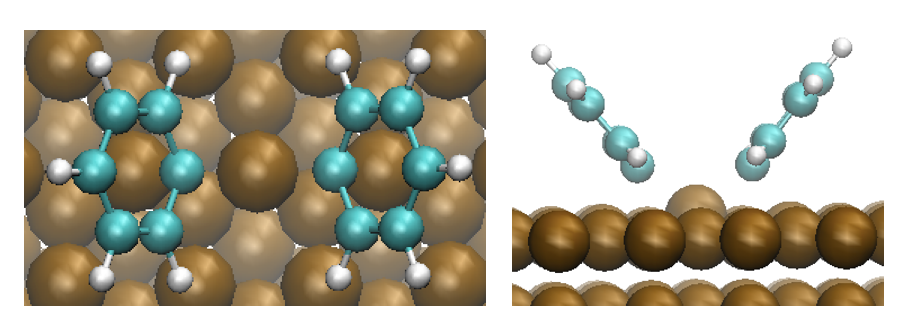
\includegraphics[width=0.45\textwidth]{Fig/organometallicintermediate.png}
%\caption{The organometallic intermediate on Cu(111) surface}
%\label{fig:organometallicintermediate}
%\end{figure}

\subsection{Formation of Carbon Carbon (C--C) Bond}

{\color{blue}
The final step is the formation of C--C bond. As discussed above, we explored the two possible pathways to construct C--C bond from C--Cu--C bridge intermediate structure (IM4). In the first pathway (Path I), the \emph{ideal surface} Cu atom will return to its original position in the first layer once the C--C bond is formed without creating an adatom. In the second pathway (Path II), the \emph{ideal surface} Cu atom is fully pulled out and become an \emph{extracted adatom}, with leaving a vacancy in its original position. %This means that the metal atom is of $nature(1)$ at the beginning of surface Ullmann coupling, and in the end it changes to $nature(2)$ through the $origin(2)$ method, becoming a new adatom on metal surface.
Here, we investigated two possibilities separately.
}
\subsubsection{Path I: ideal surface Cu returns to original location after Coupling Reaction}

{\color{blue}
The green line in Fig.~\ref{fig:completeenergy} shows path I. 

Fig.~\ref{fig:bondformlift} demonstrated the NEB calculation data and geometry transformation from C--Cu--C bridge intermediates (IM4) to final dimer on a perfect surface (Dim-g) along the green path. 
$\Delta E$ and $E_{barrier}$ of this step are \SI{-2.00}{\electronvolt} and \SI{0.49}{\electronvolt}. Experiment has indicated that the onset temperature for this step is above \SI{300}{\kelvin}~\cite{sur_sci01}, which is in line with the calculated $E_{barrier}$.
This step has been investigated previously, $\Delta E$ and $E_{barrier}$ are provides as \SI{-1.90}{\electronvolt} and \SI{0.38}{\electronvolt} based on a smaller slab and same DFT functional.
The Cu atom is back to the first layer from \SI{0.56}{\AA} height above in this step. The distance between two carbon atoms which are going to construct a covalent bond starts from \SI{3.10}{\AA}, then shortened by \SI{0.82}{\AA} in the transition state and finalize in \SI{1.49}{\AA}, which is the C--C bond length in biphenyl molecule. The change of this distance is consistent with earlier work~\cite{sur_sci01}. The tilt angle of phenyl ring with respect to copper surface varied from \SI{52}{\degree} to \SI{34}{\degree} and ends in nearly \SI{0}{\degree}.
}

%R1111: LATER. We need to develop better notation for all chemical species and refer to them consistently.
%R1111: comparison to existing calculations. Comparison between different metals (and halogens?) in our own calculations. (%ZZ the energy change is the same for halogens(halogens are not involved))
In Path I, the formation of C--C bond started from the dimerized organometallic intermediate in which the copper atom was partially lifted (notated as $IS_{path1}$). Then the two carbons which would construct a new bond later slope closer to each other, while the copper atom was less lifted on the surface (notated as $TS_{path1}$). Finally, a new C-C bond was formed and the surface went back to original configuration, no adatom forms after the coupling reaction finished (notated as $FS_{path1}$).

%In Fig.~\ref{fig:bondformlift}, along the potential energy surface, 6 intermediates were interpolated between $IS_{path1}$ and $FS_{path1}$. The tilt angle of phenyl species in respect to the Cu(111) surface was $50^\circ$ in $IS_{path1}$ and flattened to $35^\circ$ in $TS_{path1}$ and ended at $0^\circ$ in $FS_{path1}$. The distance between the two carbon atoms which would construct a bond varied from 3.10~\si{\angstrom} to 2.28 \AA\ and ended at 1.49 \AA\.

In Fig.~\ref{fig:bondformlift}, along the potential energy surface, 6 intermediates were interpolated between $IS_{path1}$ and $FS_{path1}$. The tilt angle of phenyl species in respect to the Cu(111) surface was 50\si{\celsius} in $IS_{path1}$ and flattened to $35^\circ$ in $TS_{path1}$ and ended at $0^\circ$ in $FS_{path1}$. The distance between the two carbon atoms which would construct a bond varied from 3.10~\si{\angstrom} to 2.28~\si{\angstrom} and ended at 1.49~\si{\angstrom}. 

Path I reaction is exothermic, the enthalpy $\Delta H$ is -2.00~\si{\eV}, and $E_{barrier}$ is 0.50 eV.
%R1111: This results agree with the computational study of the C--C formation of dibromobenzene species. Reference.

%R1111: LATER. It is important to discuss the zero-energy for this step. Would it be more informative to use a common zero from the entire energy profile?
\begin{figure*}[hbt]
\centering
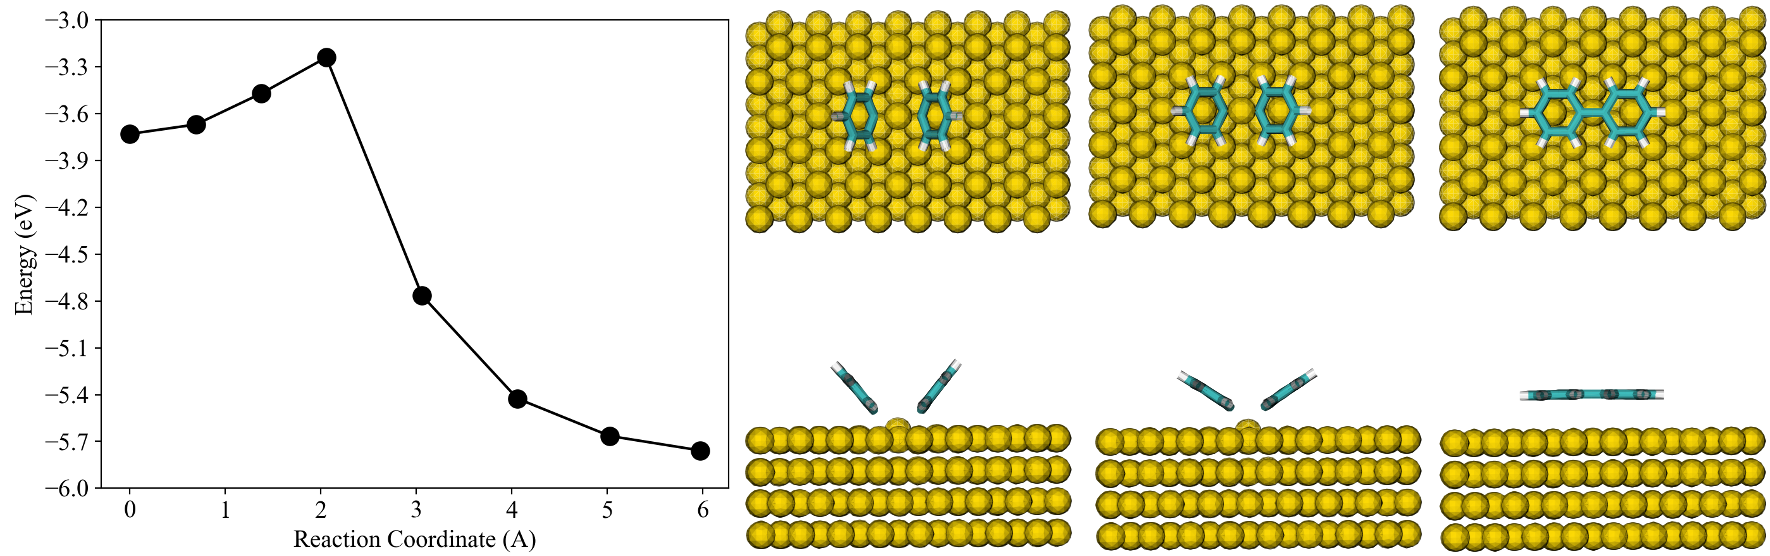
\includegraphics[width=1.0\textwidth]{Fig/bondformlift.png}
\caption{C-C bond formation through lifting Cu atom Path I}
\label{fig:bondformlift}
\end{figure*}


\subsubsection{Path II: Cu becomes a new adatom after coupling reaction}

{\color{blue}
The red line in Fig.~\ref{fig:completeenergy} shows the path that in an \emph{ideal surface} Cu atom is fully extracted by the C--Cu--C bridge intermediates out of the first layer and become a \emph{new formed adatom} with the formation of C--C bond. There exists two consecutive reactions in this path, the two transition states are explored individually. 

Fig.~\ref{fig:IM4_TS} shows first trajectory from IM4 to the C--Cu--C bridge intermediates with a fully extracted Cu adatom (IM-r1). In IM-r1, there is a vacancy on the original location of \emph{newly formed adatom}. 
$\Delta E$ and $E_{barrier}$ of the first step are \SI{-0.20}{\electronvolt} and \SI{1.38}{\electronvolt}. The distance between carbons inside C--Cu--C bridge structure increases to \SI{3.89}{\AA} (in IM-r1) from \SI{3.10}{\AA}, and cuts down by \SI{0.34}{\AA} in the transition state. The tilt angle flattens to \SI{13}{\degree} from \SI{34}{\degree}.

Fig.~\ref{fig:bondformadatom} displays the NEB energy diagram and the key intermediates configurations from IM-r1 to dimer formed on top of the \emph{newly formed adatom} (Dime-r1).
$\Delta E$ and $E_{barrier}$ of this step are \SI{-0.17}{\electronvolt} and \SI{2.01}{\electronvolt}. It ends in the formation of a new covalent C--C with a bond length at \SI{1.50}{\AA}, the former distance between these two carbons is \SI{3.10}{\AA} in IM-r1, and condenses by \SI{0.57}{\AA} in transition state. The tilt angle in Dim-r1 is a little twisted to \SI{-9.1}{\degree}. The configuration of biphenyl should be a nearly plane structure, this can be explained by the fact that the new formed C--C is directly on the top of fully extracted Cu adatom. The distance from the Cu adatom to formed C--C bond is \SI{1.66}{\AA}, leading to the repulsion force and distort the two phenyl ring to a degree.
This path will finally reach the state where a new adatom, a vacancy spot and a biphenyl form on copper surface. Ideally there are no interaction among these three species (Dim-r2). The energy of Dim-r2 is increased by \SI{0.14}{\electronvolt} compared to Dim-r1.

Besides, we also investigated the effect of Ullmann coupling intermediates on creation of adatoms, as shown in Fig.~\ref{fig:onlysurface}. The bottom line shows the potential energy of IM3, IM4 and IM-r1 in Fig.~\ref{fig:completeenergy}. The surface configuration of these three intermediates are separately taken out from the system and perform a single point energy calculation, the results are displayed in the top line. The energy of copper surface increased by \SI{1.48}{\electronvolt} from IM4 to IM-r1, but the potential energy of IM-r1 is \SI{0.20}{\electronvolt} lower than IM4, this means that the interaction between two phenyl species and the \emph{ideal surface} Cu is strong to extract the Cu atom out of first layer, and even lead to a more stable state on potential energy surface.

}


In Path II, the process started from the organometallic intermediate whereh the copper atom is fully pulled out as an adatom (notated as $IS_{path2}$) (here we created a vacancy on surface corresponding to the creation of adatom, to assure the whole system has the same number of atoms). Then the two phenyl groups would be lifted higher and closer to each other, while the copper atom is less lifted and move towards a hollow site on the surface(notated as $TS_{path2}$). Finally, a new C-C bond is formed and a new adatom and a new vacancy are created on the surface (notated as $FS_{path2}$).

As Fig.~\ref{fig:bondformadatom} show, in this path, 10 intermediates were interpolated between $IS_{path2}$ and $FS_{path2}$.The tilt angle of phenyl species in respect to the Cu(111) surface initialized at $8.5^\circ$ and $12.2^\circ$ in $IS_{path2}$ (the difference angle could be accounted by the fact that vacancy is close the one phenyl species, this will affect a little on the tilt angle), then flattened to nearly $0^\circ$ in $TS_{path2}$ and ended at $-9.1^\circ$ in $FS_{path2}$ (the negative angle arises from the fact that the adatom is right behind the biphenyl). The distance between the two carbons which would construct a bond varied from 3.89 \AA\ to 2.53 \AA\ and ended at 1.50 \AA\ .

Path II reaction is slightly exothermic, the enthalpy $\Delta H$ is -0.17 eV, and $E_{barrier}$ is 2.00 eV, higher than the $E_{barrier}$ of Path I.

\begin{figure}[hbt]
\centering
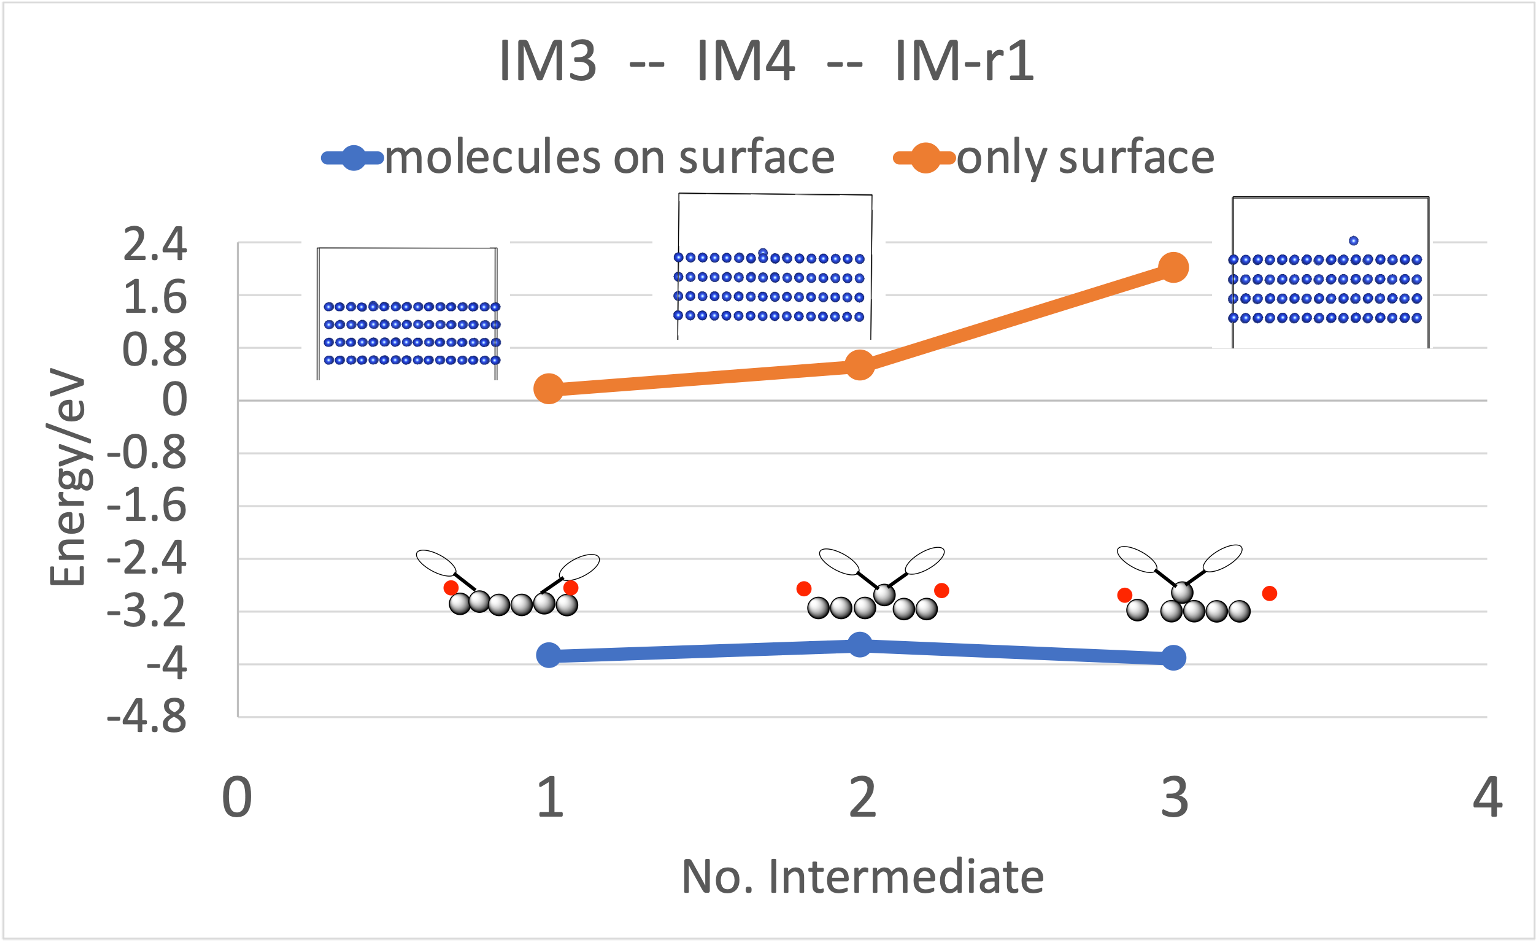
\includegraphics[width=0.45\textwidth]{Fig/onlysurface.png}
\caption{Energy diagram of IM3, IM4 and IM-r1, top line is the energy of pure surface geometry and the bottom line is the energy of Ullmann reaction species on surface.}
\label{fig:onlysurface}
\end{figure}

\begin{figure*}[hbt]
\centering
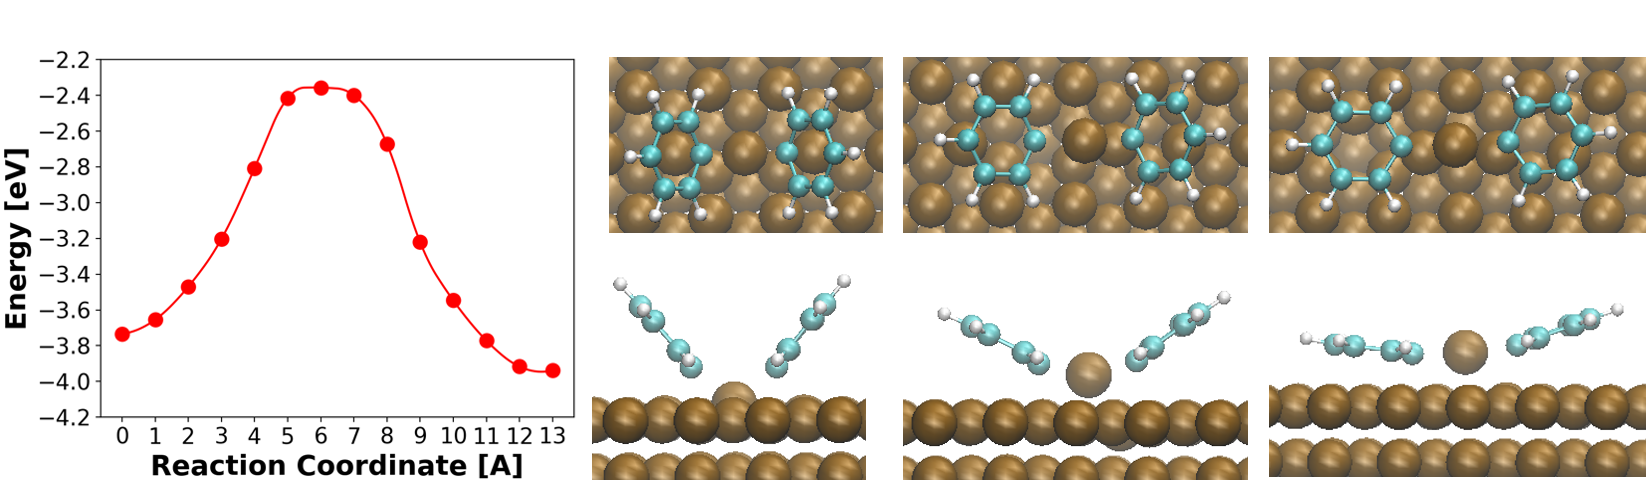
\includegraphics[width=1.0\textwidth]{Fig/IM4_IM_r1.png}
\caption{Full extraction of an ideal surface Cu atom out in Path II}
\label{fig:IM4_TS}
\end{figure*}

\begin{figure*}[hbt]
\centering
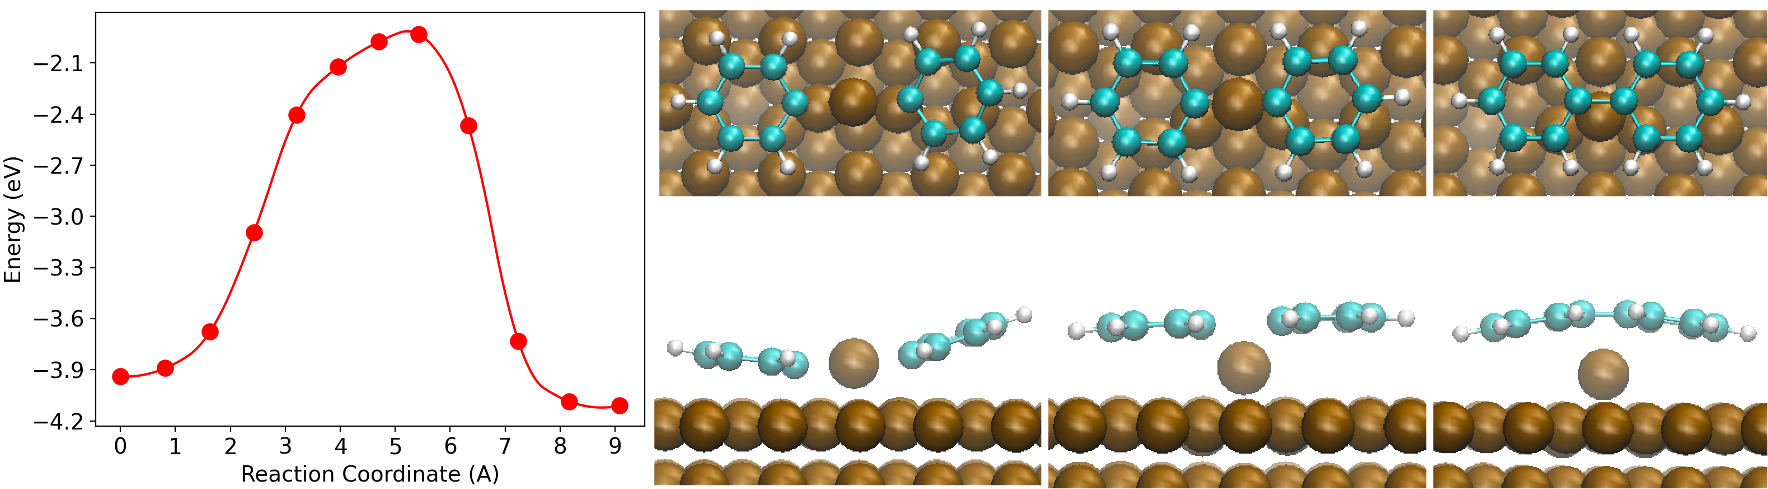
\includegraphics[width=1.0\textwidth]{Fig/bondformadatom.png}
\caption{C-C bond formation through new formed adatom Path II}
\label{fig:bondformadatom}
\end{figure*}

%R1111: All titles and subtitles use sentence case, meaning only the first word is capitalized.
\subsubsection{Path I vs path II}

{\color{blue}
The possibility of path I and path II are compared in multi-dimension.
The potential energy data and simplified geometry are present in Fig.~\ref{fig:completeenergy}. Two mechanism start to vary from IM4, path red is both kinetically and thermodynamically more favourable due to a lower-energy transition state and more stable product. This means at the same temperature condition, the reaction indicated in path I will take place at a higher speed and account for a larger percentage.

However, the evidence in geometry provides a different result. In experiment, the distance between two carbons in C--Cu--C bridge structure is \SI{4.5}{\AA} \textpm\ \SI{0.6}{\AA} based on the STM image of this bridge intermediates. This corresponds to the distance in IM-r1 of path II, which is \SI{3.89}{\AA}. This means that the C--Cu--C intermediates is more likely to possess an adatom in nature, this adatom is either from an \emph{ideal surface} or it is an \emph{pre-existing} adatom.

Taking the reaction condition into consideration. The temperature of final forming C--C bond from two phenyl species need to go up to above \SI{300}{\kelvin}~\cite{sur_sci01}. The activation energy of IM4 evolved to TS-g in green line and to TS-r1 in red line are \SI{0.38}{\electronvolt} and \SI{1.38}{\electronvolt}, respectively. The experimental temperature can meet the requirement of both two paths, but the reaction in path II will occur with a higher speed.

}
Taking the data of Path I and Path II into consideration, finally, a feasible C--C bond was constructed in both cases (bond length is around 1.5 \AA\, expected to be 1.34 \AA\ - 1.54 \AA). From thermodynamic aspect, Path I is much more exothermic, which means it will lead to a more stable product. Kinetically, the activation energy of Path I is also smaller than Path II, which means at the same temperature, the Path I reaction would take place at a higher speed and account for a much larger percentage. In this case, we could safely conclude that, if there is no pre-exiting adatom on copper surface, the formation of C--C bond in surface Ullmann coupling will follow the path I.

%R1111: Compare C--C distance in IM4 and IM5 to the experimental data for Ph-Halogen. Can we see IM5 experimentally? 3.89Ang vs 3.1Ang. (%ZZ: Added)


%R1111: Note that the difference between dimer1 and dimer2 is smaller than the difference between FS1 and IS. Probably because the dimer interacts stronger with the adatom than with the surface. 


\subsection{Energy diagram of complete Surface Ullmann Coupling Reaction}

{\color{blue}
The summary of thermodynamic data of all intermediates in surface Ullmann coupling reaction is present in Fig.~\ref{fig:completeenergy}.

Apart from the intermediates discussed above, we consider the desoprtion of all species on copper surface after the completion of Ullmann coupling reaction. $\Delta E$ of desorping formed biphenyl and two single bromine atoms are \SI{1.72}{\electronvolt} and \SI{4.01}{\electronvolt} in both two paths. Experiment shows that the desorption of bromine atoms on Cu(111) surface evolves above \SI{900}{\kelvin}~\cite{jacs2013}. 
}

Here taking the surface Ullmann coupling between two bromobenzene as example, the physisorption of two bromobenzene on Cu(111) surface decrease the energy of the whole system by 2.35 eV, which is widely recognized in experiment because adsorbing aromatic species on copper surface as a fast procedure. 
Then till the formation of new C--C bond, a detailed discussion has been demonstrated in previous sections. The last two successive steps are concerned with the desorption of biphenyl molecule and two dehalogenated bromine atoms. 
In total, the red line is more energetically favourable than green line, that can be considered to be a more reasonable pathway in realistic surface Ullmann coupling if there is no pre-exiting adatom on metal surface.

%%% Early steps
%R1111: LATER. Do we need adatom calculations for TS1? Perhaps only one or two halogen-metal pairs (for complete diagram). How will it affect the subsequent steps? Will the PH-Adatom roam the surface together before encountering the second Ph? PRIORITY6.
%R1111: Why there is no Cu-atom lifting during the C-X bond dissociation? Compare to previous works. Actually partial lifting is a process with a barrier for Au and Ag surfaces but not for Cu. We might need to reproduce this after all. --> More comparison to the existing calculation is required.

%%% Late steps
%R1111: Is the later part of the diagram halogen independent? YES!
%R1111: The barrier between IM4 and IM5 is important. Because it seems that it exists when the adatom is pulled by the R-X dissociation. PRIORITY2. Use NEB to find it.
%R1111: We need free energy for the important IM4->IM5 step. This will include increased entropy of the adatom-vacancy system (assuming that the atom with two phenyls diffuse freely). PRIORITY4.
%R1111: What is the energy of the state after dimer1, when the dimer "falls" flat to the surface? It should be around -3.97 eV. dimer1-2: dimer2+fs1-IS-IS=-3.97 eV
%R1111: An alternative TS2-1 must be calculated. The final product should be lying flat on the surface. PRIORITY3.
%R1111: What effect is responsible for the energy lowering upon adatom creation in IM5? Note that for I--Ph on Cu the extraction+diffusion during the C-I breaking step produces the overall uphill step. PRIORITY1. Remove Ph in IM3, IM4, IM without geometry relaxation (only the metal surface, not phenyl).

%%% Minor comments
%R1111: State labeling is poorly planned. Relabel states to stick to one system.
%R1111: Should we add one more TS between IM2 and IM3? LATER.
%R1111: How does the vacancy affect the energy? LATER.
%R1111: Halogen filling the vacancy or sitting on top of the adatom? PRIORITY5.

%RZK1222: This important effect needs to be properly described. The height of TS2-1 means that IM5, once formed will not undergo the C--C bond formation and can be viewed as an undesirable by-product of the reaction (unless it exists in quick equilibrium with IM4, which can be entropically hindered -- hard to find that vacancy again).

%RZK1222: How difficult is it to push the adatom (with attached organic radicals) DOWN?

\begin{figure*}[hbt]
\centering
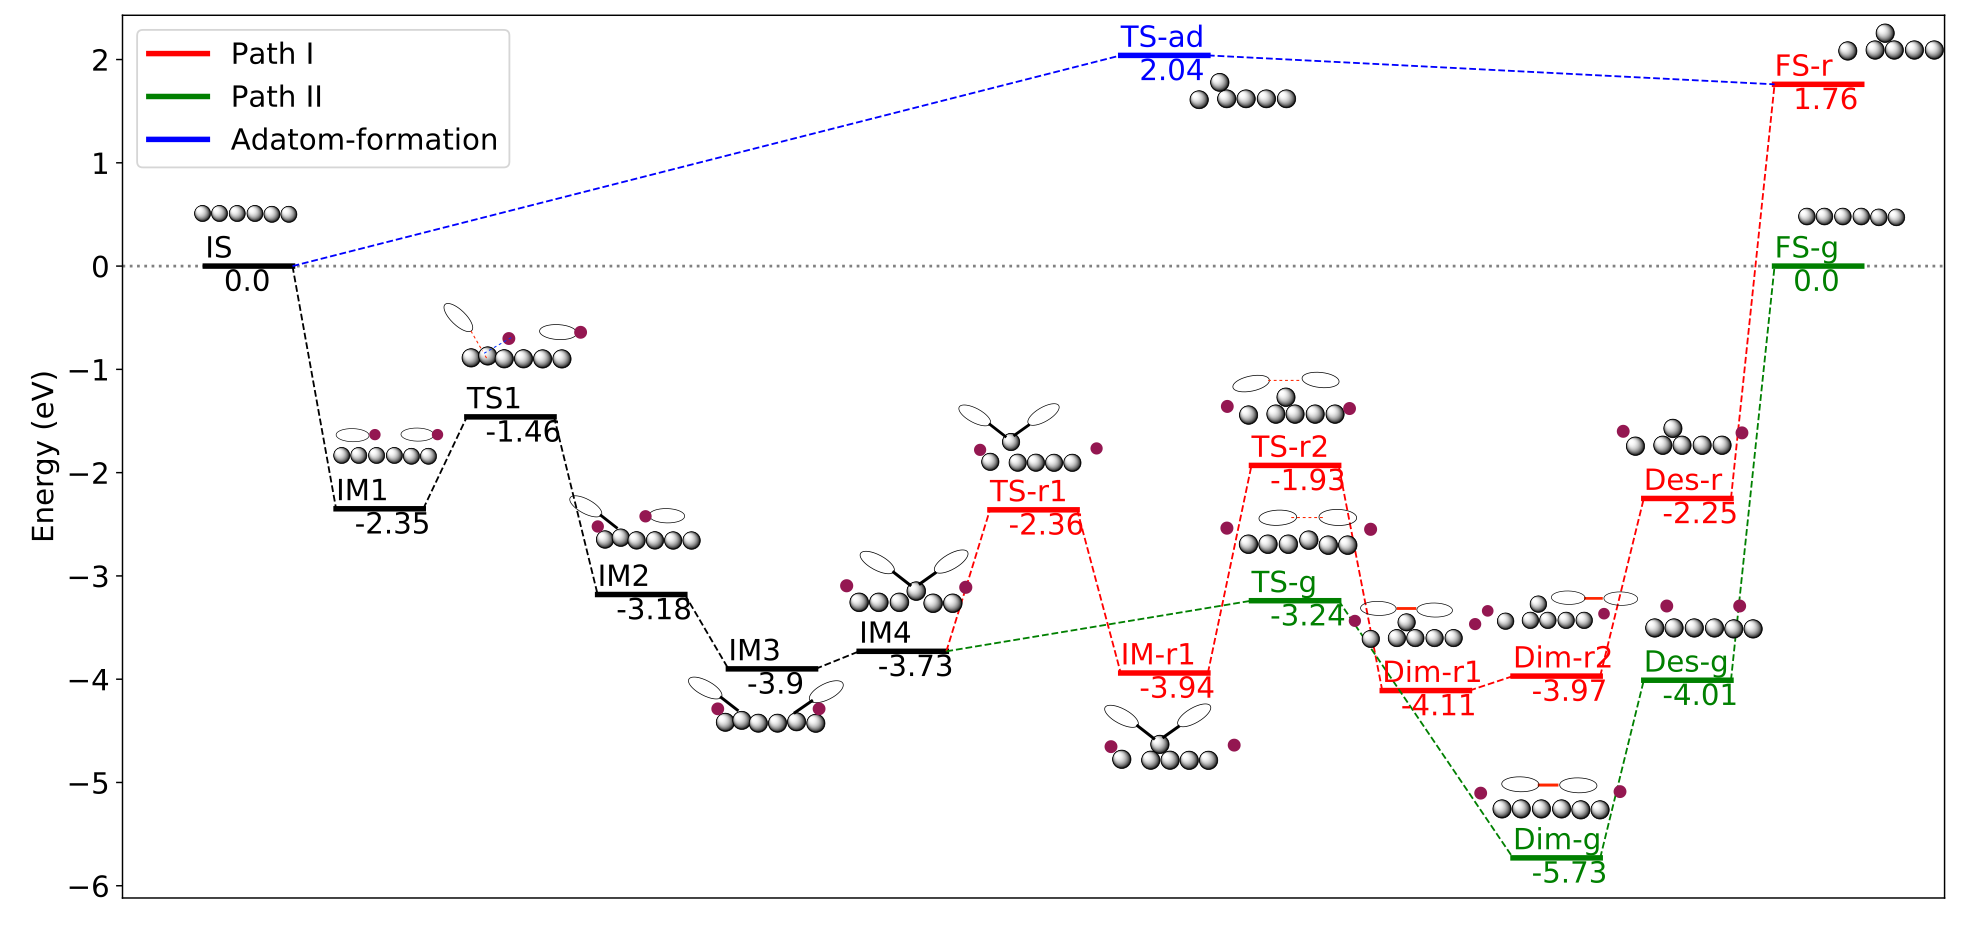
\includegraphics[width=0.98\textwidth]{Fig/completeenergy.png}
\caption{The Energy Diagram of Surface Ullmann Coupling Reaction.
the red line is the surface Ullmann Coupling reaction following Path II, the green line is following Path I. Finally, red line ended with a adatom-vacancy pair on Cu(111) surface and the green line ended same as the original Cu(111) surface.(red circle means bromine atoms)}
\label{fig:completeenergy}
\end{figure*}

\subsection{Formation of Adatom on Pure Cu Surface}

{\color{blue}
Finally, the energy of forming an adatom on a perfect Cu(111) surface is also presented. The goal of showing this energy diagram is to launch a comparison between two different conditions both delivering an adatom on Cu(111) surface. One is the formation without any species on metal surface, the other one is with surface Ullmann coupling reaction.
As Figure.~\ref{fig:pureadatomform} shows, the reaction of forming a new adatom-vacancy pair on perfect Cu(111) surface is endothermic, $\Delta H$ is 1.76 eV and the $E_{barrier}$ is 2 eV. This means at room temperature, the formation of adatom is unfavourable. 
However, as is shown in Fig.~\ref{fig:completeenergy}, the presence of organometallic intermediate in surface Ullmann coupling could promote the formation of adatoms on surface both thermodynamically and kinetically. This pathway might be considered as a plausible method to create adatoms on metal surface.
}
\begin{figure*}[hbt]
\centering
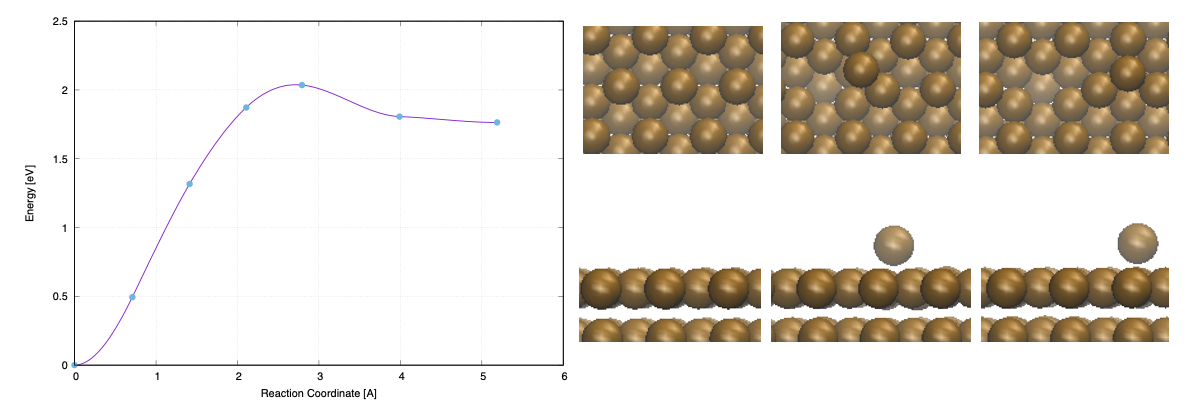
\includegraphics[width=1.0\textwidth]{Fig/pureadatomform.png}
\caption{adatom formation on pure Cu(111) surface}
\label{fig:pureadatomform}
\end{figure*}

\section{conclusions}

\section{acknowledgements}

\section{Articles to read}

\href{https://doi.org/10.1016/j.apsusc.2020.145797}{Ullmann coupling of 2,7-dibromopyrene on Au(1 1 1) assisted by surface adatoms}

\nocite{*}

\bibliographystyle{apsrev4-1} % Tell bibtex which bibliography style to use
\bibliography{references}% Produces the bibliography via BibTeX.

\end{document}








